\documentclass[fontsize=12pt,paper=letter,draft=true]{scrbook}

% for 1.5 line spacing
\usepackage{setspace}
\onehalfspacing
% single spacing for table of contents
\AfterTOCHead{\singlespacing}

% recompute page layout based on the above
\recalctypearea

% more colors (like RedOrange)
\usepackage[dvipsnames]{xcolor}

% brewer qualitative colors
\definecolor{brewergreen}{HTML}{1b9e77}
\definecolor{brewerorange}{HTML}{d95f02}
\definecolor{brewerpurple}{HTML}{7570b3}

% so we can splice in PDFs
\usepackage{pdfpages}

% set up bibliography
\usepackage[
  backend=bibtex,
  minalphanames=3,
  isbn=false,
  sortcites=true,
  sorting=anyt,
  abbreviate=false,
  url=false,
  doi=false,
  maxnames=99,
  minbibnames=3,
  maxbibnames=99]{biblatex}
\addbibresource{bibliography.bib}

% enumerate* and itemize*
\usepackage[inline]{enumitem}

% for \begin{comment}
\usepackage{verbatim}

% for source-code listings
\usepackage[newfloat,draft=false]{minted}

% for formulas
\usepackage{mathtools}

% for \sfrac
\usepackage{xfrac}

% do not reset page numbers at \mainmatter
\let\mainmatterorig\mainmatter
\renewcommand\mainmatter
 {\edef\p{\arabic{page}}%
  \mainmatterorig
  % we need to compute the actual current page number. we know the page number
  % from _before_ we called \mainmatter. but what is it now? well, it is
  % certainly that +1. but we also need to account for the next chapter starting
  % on a "right" (odd) page. we do this by adding the page number modulo two.
  % TODO: double check before final version
  \setcounter{page}{\p+1+(\p-\p/2*2)}%
 }

% an environment for todos
\newenvironment{inprogress}
  {\color{brewerorange} \paragraph{\color{brewerorange} TODO}}
  {}

% a command to indicate current editing progress
\newcommand{\resume}{
  \begin{center}
    \color{brewerorange}
    \hrule
    \vspace{1pt}
    \hrule
    \hrule
    \vspace{10pt}
    \textbf{CONTINUE HERE}
    \vspace{10pt}
    \hrule
    \hrule
    \vspace{1pt}
    \hrule
  \end{center}
}

% an environment for invariants
\newcounter{invn}
\renewcommand{\theinvn}{\Roman{invn}}
\newenvironment{invariant}
  {\vspace{.5em} \color{brewerorange} \refstepcounter{invn} \noindent \textbf{\color{brewerorange} Invariant \Roman{invn}.}}
  {\vspace{.5em}}

% for handy reference
%
% paragraph without spacing:
% \setparsizes{0pt}{0pt}{0pt plus 1fil}

% additional hyphenation rules
\hyphenation{data-flow}

% in thesis: titlehead, subject, title, subtitle
\title{Noria: Partial State in Dataflow}
\author{Jon Gjengset}
\begin{document}

\frontmatter

% always arabic page numbering (default is roman in \frontmatter)
\pagenumbering{arabic}

\includepdf[pages=-]{./titlepage.pdf}
\leavevmode\thispagestyle{empty}\newpage % since title page is single-sided

\includepdf[pages=-]{./abstract.pdf}
\leavevmode\thispagestyle{empty}\newpage % since abstract is also single-sided

\section*{Prior Publication}
Much of this thesis was previously published in a conference paper~\cite{noria},
and represents the joint work of the coauthors of that paper.
\newpage

\section*{Acknowledgements}
\begin{spacing}{1}
  % TODO
  Goes here.
\end{spacing}

\tableofcontents

\mainmatter

\chapter{Introduction}

Many web applications written today are poorly served by the databases currently
available to them. The databases are too slow to sustain the application load,
and developers are forced to implement their own ad hoc caching systems to make
the database work for them. This thesis is an attempt to improve that
situation\,---\,to build a database tailored to the particulars of these
applications that provides the performance they need.

This chapter explores the thesis motivation in greater detail
(\S\ref{s:motivation}) and briefly outlines existing solutions and their
shortcomings (\S\ref{s:existing}). It then sketches out the proposed approach
(\S\ref{s:approach}) and its implementation (\S\ref{s:intro:noria}), and
provides a list of the thesis contributions (\S\ref{s:contrib}). The chapter
concludes with a road map for how to read the remainder of the thesis
(\S\ref{s:read}).

Non-technical readers should start with Appendix~\ref{s:simple} (on
page~\pageref{s:simple}).

\section{Motivation}
\label{s:motivation}

Modern web applications typically have a number of traits in common. They are
\textbf{interactive}: each incoming request has a user waiting on the other end.
They are \textbf{read-heavy}: most interactions consume content rather than
produce new content. And they experience \textbf{significant skew}: a small
number of people, posts, teams, and discussions make up the bulk of
interactions.

Such applications are usually poorly served by the traditional relational
databases that most of them use to store and query their underlying data. These
applications tend to issue the same set of read-only queries again and again,
with the underlying data changing only infrequently. Existing databases do not
optimize for this kind of workload: they run each query in
isolation\footnote{Databases query caches~\cite{mysql-query-cache,
pgpool-query-cache} cache results as long as no changes occur to the underlying
tables if queries are byte-for-byte identical. While attractive on the surface,
they often work poorly in practice when the workload is not
read-only~\cite{mysql-query-cache-nope,pgpool-query-cache}.}, and thus re-do
work that has already been done many times over. This causes reads, which are the
most frequent operation in these applications, to be slow, while writes are
simple and fast.

\begin{figure}
  \centering
  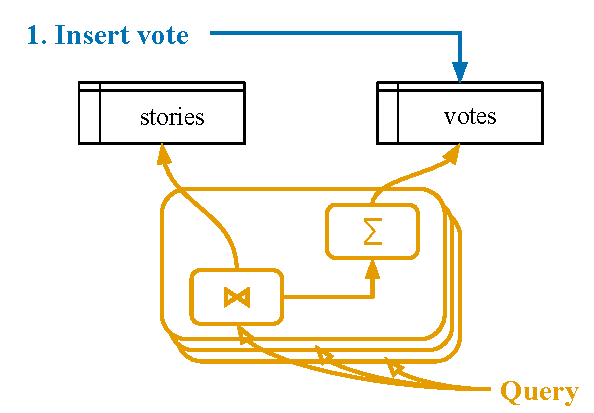
\includegraphics{diagrams/Motivation Classic DB.pdf}
  \caption{Application query execution against a traditional database. Each
  application query runs in isolation, and may perform the same work
  (\textbf{\color{set2}orange}) repeatedly. Writes do little work
  (\textbf{\color{set1}blue}), even though they are less frequent in many
  applications.}
  \label{f:motivation-classic}
\end{figure}

Figure~\vref{f:motivation-classic} shows how application queries function at a
high level in the traditional model: each query the application issues executes
the query plan, represented by an aggregation and a join in the figure. Multiple
concurrent queries execute independently, even if they run the same query.

\section{Existing Solutions}
\label{s:existing}

\begin{figure}
  \centering
  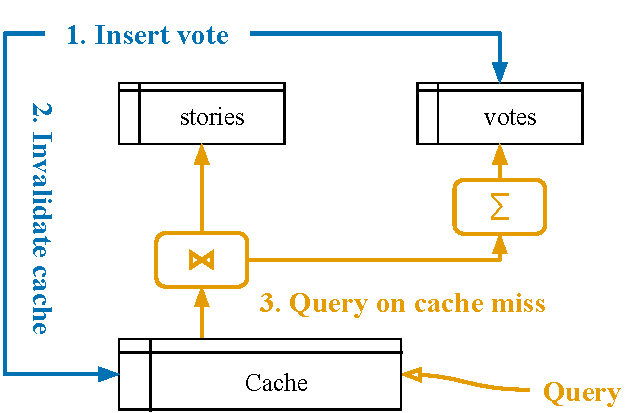
\includegraphics{diagrams/Motivation Ad Hoc Cache.pdf}
  \caption{Application query execution against a cache in front of a database.
  Application queries first check for cached results, and only execute database
  queries if the results are not cached. The application invalidates cached
  results so that later reads see the effects of new writes. The application
  logic for both reads (\textbf{\color{set2}orange}) and writes
  (\textbf{\color{set1}blue}) is more complex.}
  \label{f:motivation-adhoc}
\end{figure}

To mitigate the lackluster performance of databases for these workloads,
application authors often resort to ad hoc, error-prone
techniques~\cite{ad-hoc-caching} to exploit their applications' workload
patterns. They change their database schemas by placing and updating computed
values in the database tables, or introduce key-value stores that \textit{cache}
the result of expensive queries as shown in Figure~\vref{f:motivation-adhoc}.
All these techniques introduce significant application complexity: the
application authors must include logic to ensure that the auxiliary derived
state remains up to date as the underlying data changes, that clients do not all
flood the database when results are not available in the cache, and that
concurrent access to the database and the cache never leaves the system in an
inconsistent state.

Existing systems from industry~\cite{facebook-memcache, tao, flannel} and
academia~\cite{txcache, cachegenie, casql-consistency-thesis, pequod} have
chipped away at this problem, but are often lacking in important ways. Some
require significant developer effort, and are infeasible to implement for any
but the largest companies. Some support only a restricted set of queries, or
only provide infrastructure for developers to implement caching themselves. Many
keep the cache up to date only by evicting old results, and cannot update
existing results in-place, which is wasteful.

% Noria replaces caching \emph{logic}, not caching just caching \emph{systems}.

Eons ago~\cite{relational-materialized-views,stonebraker-views}, the database
community introduced \textit{materialized views} as an answer to the problem of
how to execute queries that are too slow to execute on demand. Materialized
views store the contents of \textit{views} (i.e., named queries) which makes
those queries faster to execute~\cite{materialized-views}. The materialized
views can then be \textit{maintained} incrementally, meaning results are updated
in-place, rather than invalidating stored results or re-executing queries from
scratch when the underlying data changes~\cite{materialized-survey}.

\begin{figure}[h]
  \centering
  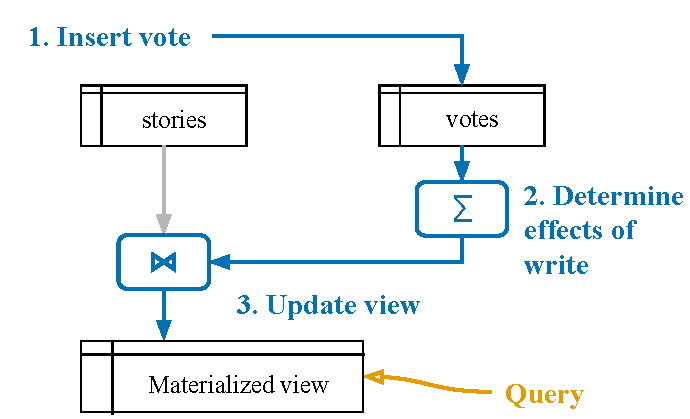
\includegraphics{diagrams/Motivation Materialized Views.pdf}
  \caption{Application query execution against a materialized view. Application
  queries only hit the view, which gives simple yet fast reads
  (\textbf{\color{set2}orange}). The database must determine the effects of
  every write and update the views to reflect changes
  (\textbf{\color{set1}blue}).}
  \label{f:motivation-materialized}
\end{figure}

Figure~\vref{f:motivation-materialized} shows an approximate architecture for an
incrementally-maintained materialized view system. The system updates the
materialized results in response to application writes, and reads access only
the stored results. Sadly, few commercially available databases support
materialized views, and the ones that do have significant
restrictions~\cite{mssql-materialized-view-restrictions}.

State-of-the-art research systems support flexible materialized
views~\cite{dbtoaster,materialize}, but do not support low-latency reads. In
these systems, reads cannot access the materialized view directly, and must
synchronize with the write-processing pipeline to get query results. Many of
these systems are also restricted to a predeclared set of queries, and cannot
incorporate changes to application queries without restarting.

Most materialized view systems do not have the ability to evict infrequently
accessed state that accumulates over time. They thus function poorly as a
replacement for a cache: infrequently accessed results cannot be evicted, and
reads must wait on writes. Dynamic materialized
views~\cite{dynamic-materialized-views, partially-materialized-views} allow the
application to materialize only a subset of each view. This enables limited
eviction, but is cumbersome for the application to manage, and only allows
coarse-grained eviction decisions (\S\ref{s:disc:emulating}).

\section{Approach: Partial State}
\label{s:approach}

Materialized views represent an ``almost there'' solution to automatic caching.
They provide a great foundational mechanism for storing and maintaining query
results efficiently in a way that meshes well with how applications already
work: by issuing SQL queries. What is missing to make materialized views a
viable replacement for the ad hoc caching strategies today's applications employ
is a way to make the materialized views more dynamic. Specifically, to serve as
a good cache-substitute, materialized views must support efficiently adding new
queries and evicting old results at runtime.

To bridge the gap, this thesis proposes \textit{partially materialized
state}\footnote{The database literature sometimes refers to a view where only
some columns are materialized as ``partially
materialized''~\cite{partially-materialized}. This meaning of the term is
unrelated to the use of the term in this thesis.}, or partial state for short.
Partial state lets entries in materialized views be marked as \textit{missing},
and introduces \textit{upqueries} to compute such missing state on-demand.
This allows new queries to be added efficiently by leaving the initial
materialized view empty, and populating the view only in response to application
queries. Furthermore, as the application loses interest in old query results,
those results can be evicted to reclaim memory, which can in turn be used to
cache more important query results. In essence, partial state enables
materialized views to function like caches.

In the proposed work, the system model still looks like
Figure~\vref{f:motivation-materialized}, except that the materialized view also
contains parameters whose value the application supplies at runtime. Queries to
the materialized view can then \emph{miss} for a given parameter value, just
like in a cache. When they do, the database internally fills in the missing
state before it responds to the application. If the application later executes
the same query, the cache holds the result. Over time, the database evicts
infrequently accessed results to save memory and to avoid the overhead of
maintaining results the application is no longer interested in.

\section{Partial State in Noria}
\label{s:intro:noria}

The thesis includes an implementation of partial state in Noria, a
state-of-the-art materialized view system that is already optimized for
read-heavy, dynamic web applications~\cite{noria}. Noria uses \textit{dataflow}
internally to maintain its materialized views, a system architecture that allows
fast and distributed computation over a stream of data changes. Dataflow
represents computational dependencies as a directed acyclic graph where edges
represent data dependencies, and vertices represent computations (like
aggregations or joins) over the data that arrives over the incoming edges.
Partial state upqueries flow ``up'' this dataflow, in the opposite direction of
the data, and trigger the retransmission of past state in the case of a cache
miss. The resulting retransmissions then use the existing Noria dataflow to
process the responses and fill in missing state. This avoids the need for
separate logic for serving cache misses and maintaining already cached state,
and simplifies the implementation.

\section{Contributions}
\label{s:contrib}

The main contributions of this thesis are:

\begin{itemize}
 \item A model for, and implementation of, partial state in a dataflow-based
   materialized view system.
 \item Upqueries\,---\,a mechanism that populates missing state on demand.
 \item An analysis of the inconsistencies that arise when introducing partial
   state to a distributed, high-performance stateful dataflow processing system
    where updates can race with one another, and with upqueries.
 \item Techniques for overcoming those inconsistencies while preserving system
   correctness, performance, and scalability.
 \item Micro and macro evaluations of the performance and memory benefits of
   partial state. Experimental results suggest that the presented system
    increases supported application load by up to $20\times$ over MySQL, and
    reduces memory use by up to $\sfrac{2}{3}$ compared to existing approaches.
\end{itemize}

\section{Reading Guide}
\label{s:read}

The rest of the dissertation is organized as follows: Chapter~\ref{s:noria}
describes the Noria dataflow system. Chapter~\ref{s:partial} introduces the
partially stateful dataflow model. Chapter~\ref{s:correct} describes additional
mechanisms that are needed to ensure that partially stateful dataflow produces
correct query results. Chapter~\ref{s:impl} details some of the implementation
decisions in the thesis prototype. Chapter~\ref{s:eval} evaluates Noria's
implementation of partial state on a realistic application query workload.
Chapter~\ref{s:related} explores related work. Chapter~\ref{s:disc} discusses
shortcomings of, and alternatives to, partial state. Finally,
Chapter~\ref{s:future} outlines future work on partial state.

For readers that are unfamiliar with database queries, materialized views,
dataflow, and application caching, but would still like to understand roughly
what this thesis is about, Appendix~\ref{s:simple} starting on
page~\pageref{s:simple} is for you.


\chapter{Background \& Related Work}

This chapter provides introductory background information on many topics that
are relevant to the work in this thesis, as well as an overview of existing
systems and their relation to Noria and partial state.

\section{Materialized Views}

Noria's primary function is to provide materialized views. In database parlance,
a \textit{view} is a name for the result set of a particular query. When an
application reads from a view, it is reading from the result set that results
from executing that query. Most databases also allow views to be used in place
of other database collections, like tables, in other queries.

Some databases can \textit{materialize} a view by storing the result set
somewhere for later recollection. When a view is materialized, queries over that
view do not re-execute the view's backing query, but instead access the rows of
the view as if they were stored in a durable database relation. Materialized
views thus effectively provide query memoization; they are faster to access than
non-materialized views, at the cost of having to store the view's rows.

Once a database materializes a view, it must \textit{maintain} that
materialization over time as the underlying data changes. Otherwise, reads from
the view would no longer match the results of the view's backing query. View
maintenance can be \emph{reactive} by updating the view as the data changes,
\emph{demand-driven} by updating the view only when queried, or \emph{triggered}
by updating the view only when an outside trigger is invoked.

Noria implements reactive view maintenance\,---\,it assumes that writes are less
frequent than reads, and therefore that it is better to make writes slower by
updating the cache proactively than to make reads slower by having each read
check that the materialization is up to date.

\paragraph{Materialization.}
Throughout this thesis, the word materialization is often used as a noun. In the
context of Noria, a materialization refers to any derived computation result
that Noria explicitly stores, not just materialized views. Or, more precisely,
Noria may choose to materialize intermediate results, such as the current value
of an aggregation, which do not represent any of the application's queries.
These intermediate materializations are still views\,---\,they have a schema and
consist of rows\,---\,but do not reflect any named views that the application
has created.

\subsection*{Related Work}

Database materialized views~\cite{gupta-view-selection,lee} were originally
devised to cache expensive analytical query results. Unfortunately, commercial
databases' materialized view support is limited, and views must usually be
rebuilt from scratch when the underlying data
changes~\cite{materialized-view-selection-sql-server,mssql-materialized-view-restrictions-blog,
mssql-materialized-view-restrictions}.

The key to usable materialized views is how they are maintained incrementally as
the underlying data changes, which has been the subject of considerable research
in the past few decades. \citeauthor{materialized-survey} gives a good survey of
the current landscape in \cite{materialized-survey}.

Modern incremental view maintenance (IVM) techniques are usually based on
\textit{delta queries}, which are algebraically derived queries that give
efficient relational expressions for computing the change to a (materialized)
view given a set of changes to the underlying data. The current state-of-the-art
in IVM is \textit{Higher-Order IVM}, in which the system derives multiple,
recursive such delta queries for each view, and strategically materializes and
maintains the intermediate delta query results as well~\cite{dbtoaster, hotdog}.
Recent work also proposes techniques for mitigating the memory overhead of such
intermediate materializations by instead materializing smaller auxiliary state
from which the necessary values can then be efficiently produced when
needed~\cite{memory-efficient}. Sadly, few of these solutions have been adopted
in commercially available databases.

Noria's dataflow for each view are effectively delta queries for that view over
the stream of updates to base tables. Noria's current algorithms for what
dataflow to use to compute the changes to each view are fairly naive, and could
likely benefit from the techniques in the aforementioned work. However, Noria
does apply some of the lessons from higher-order delta queries, and also
materializes intermediate results to speed up the delta processing. Meanwhile,
Noria's dataflow-backed processing provides a significant benefit by virtue of
using the dataflow model. In particular, it allows Noria to easily distribute
the view maintenance across cores and machines to improve performance.
Furthermore, Noria is designed to take advantage of a relaxed consistency model,
which allows much higher read performance than strongly consistent systems can
provide.

Through the work of this thesis, Noria also supports \emph{partial} view
materialization, which allows it to materialize and maintain only a subset of
each of the application's views. This is not possible in most existing IVM
systems. Pequod~\cite{pequod} and DBProxy~\cite{dbproxy} support partial
materialization in response to client demand, although Pequod is limited to
static queries specified in a datalog-like language, and DBProxy does not
support incremental view maintenance. And neither system shares state nor
processing across views.

\section{Caching}

As applications grow, their performance needs often exceed that which a
traditional relational database can provide. Such applications cannot afford to
wait for the database to compute joins and aggregations, and need lower-latency
data access than a relational database like MySQL or Postgres typically
provides. In these cases, application authors tend to add \textit{caching} to
their application backend logic.

Caching is a broad topic, especially because caching tends to occur at multiple
levels within the application. Developers may cache results of individual
database queries, collections of data that the application frequently uses
together, computed and otherwise derived values that are expensive to
re-compute, segments of rendered application output (like HTML snippets), all
the way to full web pages. Each of these caches may also exist in multiple
places to improve data locality, add redundancy, or simply because two caches
partially overlap.

Noria implements \textit{query result caching} (using materialized views), which
ensures that the application's database queries are fast, even if they are
complex or include significant computation. While Noria could likely be extended
to maintain the compound caches higher up in the application stack, that is left
for future work.

Much like with view materialization, the introduction of a cache requires that
the application maintains those caches such that new data eventually becomes
visible. The exact mechanism that is used to implement the cache maintenance
varies by cache type, developer preference, and application size.

Once a cache is in place, the application authors must also implement cache
\textit{eviction} to ensure that the cache does not grow without bound. Many
eviction strategies exist, and revolve around the notion that certain cache
entries are more worthwhile to keep than others. These entries are usually
referred to as ``hot'' entries. Essentially, if storage space is limited, it is
likely better to keep hot a cache entry that is accessed once a second than a
``cold'' entry that was last accessed two weeks ago. \textit{Partial state}, the
topic of this thesis, is what allows Noria to implement eviction for
materialized views.

\subsection*{Related Work}

Application-level caching is often implemented in an ad-hoc fashion, and tends
to be the source of many application errors~\cite{ad-hoc-caching}. Researchers
and industry teams alike have therefore attempted to build systems to automate
cache maintenance.

Large-scale applications often end up building their own custom caching
infrastructure~\cite{facebook-memcache, flannel}, which solves their needs in
isolation, but does not provide a ready-to-use solution for other application
developers that face similar issues. These custom-built solutions also tend to
implement only the minimum functionality the authors need at the time, and
forego more complicated, but nonetheless useful features such as incremental
cache updates.

The research community has also produced several systems that aim to provide
more general-purpose transparent caching. TAO~\cite{tao} and
TxCache~\cite{txcache} implement automated query result caching, but do not
support incremental in-place cache updates. CacheGenie~\cite{cachegenie}
implements a trigger-based middleware cache for object-relational mapping
frameworks, and supports in-place cache updates, but is limited to only specific
operations supported by the framework.

In the world of database literature, database caching frontends are sometimes
referred to as \textit{Cache-Augmented SQL} systems. And there, like with all
caching systems, the primary concern is one of consistency\,---\,\emph{some}
mechanism must be in place to ensure that the cache remains up to date as the
underlying data changes. Research in this space tends to focus on cache
management as being external to the database, and augments the key-value store
used to store the cache entries so that this external system can correctly
manage the race conditions that arise when the database and cache are distinct
systems~\cite{facebook-memcache, casql-consistency, casql-consistency-thesis}.
Noria instead integrates the cache management into the database, which allows
the cache entries to be incrementally updated, automatically, in-place.

A related approach is \textit{mid-tier database caching}, in which subsets of
the database are replicated onto the hosts that run the application's code. This
allows certain queries to be run locally without interacting with the remote
database backend~\cite{mtcache}. While the approach is appealing in that some
database queries can avoid traversing the network, it does not provide the same
speedups that query result caching provides.

\section{Dataflow}

Noria maintains its materialized views using \textit{dataflow}. Dataflow means a
thousand things to a thousand people, especially if they are from different
areas of computer science, but this thesis will focus on dataflow as understood
in software computing specifically. Even there, many definitions exist, but they
all agree that in dataflow, compute is stationary while data moves.

A dataflow system expresses complex computations as a directed \emph{graph} that
consists of interconnected nodes that implement primitive operations, such as
joins, filters, and aggregations. These nodes then \emph{stream} data among each
other to produce the desired overall results. Dataflow systems are thus also
often referred to as stream processing systems. The roots of the graph introduce
the data that the dataflow computes over, while the leaves represent the
dataflow program's outputs.

Since the dataflow model is inherently streaming, it is particularly well-suited
for distributed deployments. Nodes are independent and communicate only through
their streams, so the system can easily place them on different cores, or hosts,
and use existing messaging fabrics to connect them. If needed, nodes can also be
sharded to allow data-parallel computing.

The streaming design also makes dataflow a good fit for reactive applications.
When the data changes, the system introduces the changes at the roots, and then
observe how the leaves change in response. Those changes can in turn be
forwarded to the application to provide a change stream over the computation's
results over time.

\subsection*{Related Work}

A wide range of dataflow and stream-processing systems exist that excel at
data-parallel computing~\cite{dryad, naiad, storm, heron, flink, millwheel,
spark-streaming, stanford-stream, s-store, cloud-dataflow}. However, these
systems cannot easily serve web applications directly. They only achieve
low-latency incremental updates at the expense of windowed state (and incomplete
results) or by keeping full state in memory. Partial state allows Noria to lift
this restriction. Furthermore, these systems generally provide no mechanism for
accessing computed state except through the dataflow or by integrating with
additional external systems, which adds latency.

Many existing system are also limited to a fixed set of queries defined when the
system is started, and cannot easily adopt query changes as the application
evolves. Some dataflow systems do support Noria-like dynamic changes to the
running dataflow~\cite{ciel, ray}, but without support for demand-driven partial
state these systems must either fully compute results when the dataflow is
extended, or have new dataflow only take into account subsequent updates.

Some developers use, or consider using, a streaming fabric like Apache
Kafka~\cite{kafka} to build their own view maintenance pipeline~\cite{nyt-kafka,
samza-blogpost}. However, at the time of writing, no general-purpose system
exists based on such a pipeline that achieves the performance and flexibility of
Noria.

Differential dataflow~\cite{differential-dataflow}, and its instantiation in the
commercial product Materialize~\cite{materialize}, bears a striking resemblance
to Noria at first glance. In particular, it uses dataflow to produce
automatically-maintained materialized views over SQL queries. However,
Materialize does not implement partial state, and must therefore maintain
similar queries independently (which misses out on opportunities for shared
compute and state) or fully materialize query results (which uses more memory).
The authors behind Materialize have proposed partial solutions to some of these
challenges, which are discussed in \S\vref{s:disc:emulating}.


\chapter{Noria}
\label{s:noria}

In this thesis, partial state is implemented in Noria~\cite{noria}, a stateful,
dynamic, parallel, and distributed dataflow system designed for the storage,
query processing, and caching needs of typical web applications. Because of the
strong connection between Noria and partial state, this chapter describes the
design and implementation of Noria in sufficient depth to follow the remainder
of the thesis.

\section{High-level Overview}

\begin{listing}[h]
  \begin{minted}{sql}
/* base tables */
CREATE TABLE stories
  (id int, title text);
CREATE TABLE votes (story_id int, user int);
CREATE TABLE users (id int, username text);
/* internal view: vote count per story  */
CREATE INTERNAL VIEW VoteCount AS
  SELECT story_id, COUNT(*) AS vcount
    FROM votes GROUP BY story_id;
/* external view: story details */
CREATE VIEW StoriesWithVC AS
  SELECT id, author, title, url, vcount
    FROM stories
    JOIN VoteCount ON VoteCount.story_id = stories.id
   WHERE stories.id = ?;
  \end{minted}
  \caption{Noria program for a key subset of the Lobsters news
           aggregator~\cite{lobsters} that counts users' votes for stories.}
  \label{f:vote-src}
\end{listing}

Noria runs on one or more multicore servers that communicate with clients and
with one another using RPCs. A Noria deployment stores both \emph{base tables}
and \emph{derived views}. Roughly, base tables contain the data typically stored
persistently, and derived views hold data an application might choose to cache
to improve performance. Compared to conventional database use, Noria base tables
might be smaller, as Noria derives data that an application may otherwise
pre-compute and store denormalized in base tables for performance. Views, by
contrast, will likely be larger than a typical cache footprint, because Noria
derives more data, including some intermediate results. Noria stores base tables
persistently on disk, either on one server or sharded across multiple servers,
but stores views in server memory.

Noria's interface resembles parameterized SQL queries. The application supplies
a \emph{Noria program}, which registers base tables and views with parameters
supplied by the application when it retrieves data. Figure~\ref{f:vote-src}
shows an example Noria program for a news aggregator application where users can
vote for stories (\texttt{?} is a parameter). The Noria program includes base
table definitions, \emph{internal} views used as shorthands in other
expressions, and \emph{external} views that the application later queries. It
can be thought of as an extended schema for the application that includes its
queries. Noria supports much, but not all, SQL syntax.

To retrieve data, the application supplies Noria with an external view
identifier (e.g., \texttt{StoriesWithVC}) and one or more sets of parameter
values. Noria then responds with the records in the view that match those
values. To modify records in base tables, the application performs insertions,
updates, and deletions, similar to a SQL database. Data is represented as
structured records in tabular form~\cite{spanner, bigtable}.

Noria differs substantially from traditional databases in how queries are
executed. Rather than compute a query's results on demand when the
application executes it, Noria does so when the query view is defined.
Noria then caches, or \emph{materializes}, the contents of that view, and serves
queries to that view directly from that cache. To keep the materialized current,
Noria internally instantiates a dataflow program to continuously process the
application's writes and update the views as appropriate.

This kind of view materialization makes Noria particularly well-suited for
read-heavy applications that tolerate eventual consistency, since it shifts
query execution cost from reads, which are frequent, to writes, which are
infrequent. Noria focuses entirely on relational operators, rather than the
iterative or graph computations that are the focus of other dataflow
systems~\cite{naiad, differential-dataflow}.

The application may change its Noria program to add new views, to modify or
remove existing views, and to adapt base table schemas. Noria expects such
changes to be common and aims to complete them quickly, without restarting the
dataflow engine.

\section{Dataflow Execution}

To keep its materialized views from growing stale as the underlying data
changes, Noria uses dataflow. Noria compiles all the application queries into a
joint dataflow program, which it routes all application writes through. The
dataflow is a directed acyclic graph of relational operators such as
aggregations, joins, and filters. Base tables are the roots of this graph, and
external views form the leaves. Noria extends the graph with new base tables,
operators, and views as the application adds new queries.

When an application write arrives, Noria applies it to a durable base table and
injects it into the dataflow as an \emph{update}. Operators process the update
and emit derived updates to their children; eventually updates reach and modify
the external views. Updates are \emph{deltas}~\cite{roll, differential-dataflow}
that can add to, modify, and remove from downstream state. For example, a count
operator emits deltas that indicate how the count for a key has changed; a join
may emit an update that installs new rows in downstream state; and a deletion
from a base table generates a ``negative'' update that revokes derived records.
Negative updates remove entries when Noria applies them to state, and retain
their negative ``sign'' when combined with other records (e.g., through joins).
Negative updates hold exactly the same values as the positives they revoke and
thus follow the same dataflow paths. The combined deltas emitted by an operator
from the beginning of time constitutes the operator's current state, though this
state may not be stored anywhere.

Noria supports \emph{stateless} and \emph{stateful} operators. Stateless
operators, such as filters and projections, need no context to process updates;
stateful operators, such as count, min/max, and top-$k$, maintain state to avoid
inefficient re-computation of aggregate values from scratch. Stateful operators,
like external views, keep one or more indexes to speed up operation. Noria adds
indexes based on \emph{indexing obligations} imposed by operator semantics; for
example, an operator that aggregates votes by user ID requires a user ID index
to process new votes efficiently. Noria's joins are stateless, but require that
the state of their inputs be materialized to allow an update arriving at one
input to join with all relevant state from the other.

\subsection{Example Execution}

\begin{figure}[t]
  \centering
  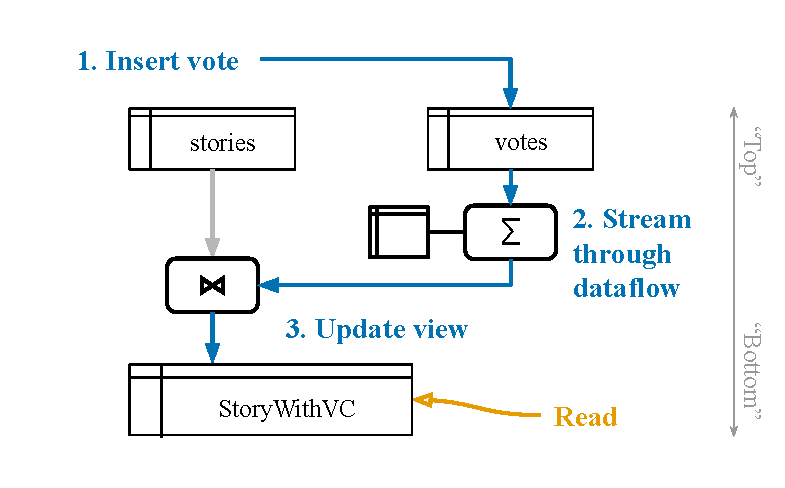
\includegraphics{diagrams/Example Execution.pdf}
  \caption{Noria's dataflow program to maintain Listing~\ref{f:vote-src}. Text
  describes the update path highlighted in blue. The dataflow inputs are
  considered the ``top'' of the dataflow, and the leaves are at the ``bottom''.
  Parents are ``upstream'' of their ``downstream'' children.}
  \label{f:example-exec}
\end{figure}

Figure~\ref{f:example-exec} shows the dataflow that Noria constructs for
maintaining the Noria program in Listing~\ref{f:vote-src}. At the top are the
entry points into the dataflow\,---\,the operators that represent the schema
base tables\,---\,one for the \texttt{stories} table, and one for the
\texttt{votes} table. Connected to the \texttt{votes} table is a counting
aggregation operator ($\sum$), which corresponds to the internal
\texttt{VoteCount} view. It then feeds into a join operator ($\bowtie$), which
in turn connects to the external \texttt{StoryWithVC} view.

To understand how Noria uses this program to maintain the external view,
consider what happens when a new vote is inserted into \texttt{votes}. The
insertion is introduced into the dataflow as a single-row update with a positive
sign at the \texttt{votes} operator. It stores the update to durable storage,
and then forwards the update as-is to its children; in this case, the count
operator.

The count operator performs a lookup into its own output state for the current
count of the new row's group by column value. The semantics of a count is that
an insertion increments that number by one, so the operator emits a replacement
update for the old state. In particular, the update it produces contains a
negatively-signed record for the old count, and a positively-signed record for
the update count. The replacement also includes the group by column value.

When the join operator receives this replacement update from the count, it
performs a lookup into its other ancestor, \texttt{stories}, for records that
match the join column value of each record of the incoming update. In this case,
both records (the negative and the positive) have the same story identifier as
the join value, so only a single record is returned\,---\,the matching story.
The operator then joins each record in the update with each matching result.
This produces an update that (still) contains one negative and one positive
record, but where each record now includes additional columns from the
\texttt{stories} table.

Ultimately, this two-record update arrives at the operator that represents the
external \texttt{StoryWithVC} view. The changes from the update are applied one
by one, with the negative record removing the entry in the view with the old
vote count, and the positive record adding the replacement entry. Once the
update has been applied, the changes are made visible to readers who will then
start seeing the updated vote count for the story in question.

\section{Consistency Semantics}

To achieve high parallel processing performance, Noria's dataflow avoids
global progress tracking or coordination. An update injected by a base table
takes time to propagate through the dataflow, and the update may appear in
different views at different times. Noria operators and the contents of its
external views are thus \emph{eventually-consistent}. Eventual consistency is
attractive for performance and scalability, and is sufficient for many web
applications~\cite{eventually-consistent, memcached-facebook, pnuts}.

Noria does ensure that if writes quiesce, all external views eventually hold
results that are the same as if the queries had been executed directly against
the base table data. Making this work correctly requires some care. For example,
like most dataflow systems, Noria requires that operators are deterministic
functions over their own state and the inputs from their ancestors. Furthermore,
operators must be distributive so that evaluating the query using
tuple-at-a-time processing is equivalent to evaluating the whole query at once.
Noria operators must also be commutative so that operators with multiple inputs,
like unions and joins, can process their inputs in any order without
coordination.%
\footnote{Maintaining eventual consistency with partial state requires
additional mechanisms, as discussed in \S\ref{s:practical}.}
The standard relational operators that Noria supports all have this property.

\paragraph{Transactions.}
Web applications sometimes rely on database transactions, e.g., to atomically
update pre-computed values. Noria does not implement transactions, though its
support for derived views often obviates the need for them. For example, web
applications often use transactions to keep denormalized schemas synchronized: a
``like count'' column in the table that stores posts or an ``average rating''
column in the table that stores products. Noria obviates the need for such
denormalizations, and the transactions needed to maintain them, by automatically
ensuring that computed derived values are kept up to date with respect to the
base data.

\section{Parallelism}

Servers have many cores, and any high-performance system must be able to take
advantage of multiple cores to take full advantage of the hardware. Noria does
so in several ways. First, it allows reads to happen independently from any
number of threads concurrently. Second, it allows different threads to process
writes in disjoint parts of the dataflow concurrently. And third, it supports
sharding individual operators, or cliques of operators, so that multiple threads
can process disjoint subsets of the data concurrently through the same dataflow
segment. These three mechanisms are described further below.

\subsection{Read Independence}

Since Noria is primarily oriented towards read-heavy workloads, its architecture
is optimized for allowing reads to go ahead at full speed whenever possible. In
particular, Noria does not synchronize reads with reads \emph{or} writes. Unless
a read encounters missing partial state, it never blocks waiting for another
thread.

This is achieved through a concurrency primitive that maintains two instances of
each materialized view, with deduplication between them. Reads go to one view,
and writes to the other. Readers only see updates to the view when a writer
exposes those changes explicitly\,---\,the writer flips an atomic pointer to the
other view, and then waits for all readers to exit the old view before modifying
it again. This can be done on every update, as Noria currently does, or only
occasionally to amortize the cross-core communication penalty. Crucially,
readers do not take locks, and generally operate only on core-local cache lines.

This design allows Noria to use any number of threads to serve reads from any
view. As long as there are cores available, new threads can be added to perform
view lookups and request serialization and deserialization.

\begin{inprogress}
  This design is further discussed in Appendix B?
\end{inprogress}

\subsection{Partitioning}

As part of dataflow planning, Noria divides the dataflow graph into a number of
sub-graphs called \textit{thread domains}. Only a single thread can process
updates in a given thread domain at a time (except with sharding; see below),
and any update that enters a thread domain is processed to completion within
the domain before another update is processed.

State is never shared between thread domains, which means no locks are needed.
Thread domains only ever communicate with one another through messages sent
across the edges of the dataflow, or in the case of upqueries, by sending
messages through dedicated upquery paths set up by the partial subsystem. All
such communication can happen either over the network if the other thread domain
is on a different host, or over an in-memory channel if it is local.

Since thread domains share nothing, some state may be duplicated across
boundaries. For example, a join operator at an incoming edge of a thread domain
must be able to perform lookups into the state of its ancestor, which sits in a
different thread domain. In such a case, Noria will create a thread-local copy
of the join's ancestor's state that it can use locally. Noria's thread domain
assignment heuristics will attempt to draw domain boundaries  such that this
kind of duplication is unnecessary. For example, it will prefer drawing a domain
boundary just before an aggregation (which does not need to look up in the state
of its ancestor), and avoid drawing a domain boundary just before a join.

\subsection{Sharding}

To accommodate applications with such a high volume of writes that the
processing at a single operator is a bottleneck, Noria supports sharding an
operator. Multiple threads split the work of handling updates to a sharded
operator, and operate like independent, disjoint parts of the dataflow.

Noria implements static hash partitioning: how an operator is sharded is
determined when it is added to the dataflow, and does not change over the
runtime of the application. Sharding by value ranges and adjusting the sharding
dynamically is left for future work.

Noria shards operators primarily based on how they access state. For example, an
aggregation performs lookups into its own state, and is sharded by the key
column of those lookups. Any other sharding would mean that processing one
update would require coordination among all shards. A join is sharded by the
join key for the same reason. Base tables are sharded by the table's primary
key. Operators that do not perform lookups (e.g., unions) continue the sharding
of their ancestors to avoid unnecessary shuffles.

To shard an operator, Noria introduces two additional nodes in the dataflow: a
\emph{sharder} placed upstream of the sharded operator, and a \emph{shard
merger} downstream of it. The sharder routes incoming updates to the appropriate
shard of the sharded operator, and the shard merger is a union operator that
combines the output of all the shards to a single downstream output stream.
Noria then eliminates unnecessary sharders and shard mergers, such as if an
operator and its ancestor are sharded the same way.

Sharding boundaries are naturally also thread boundaries, though two connected
thread domains may also be sharded differently. Or, phrased differently, Noria
may partition a chain of operators that are all sharded by the same column into
multiple thread domains to increase parallelism.

\begin{comment}
  Sharding is tracked based on "ultimately source column". (column tracing)
\end{comment}


\chapter{A Model of Partial State}

Noria without partial state, as described in \S\ref{s:noria}, uses significant
amounts of memory. All results for all queries must be materialized, and unlike
traditional caching approaches, unimportant cached results are not evicted to
free up memory. To address the high memory use of traditional materialized
views, this thesis proposes \textit{partially materialized state}. Partial state
enables Noria to store and maintain only a subset of a materialized view's
contents, and to compute missing state on demand. Partial state also enables
Noria to implement eviction, so that the materialization cost is kept low even
as the underlying workload changes.

This chapter discusses the partially stateful model and its components. The next
chapter examines the practical challenges that arise when partial state is
implemented in a dataflow system.

\section{Missing State}

Partial state allows state to be \textit{missing}. Missing state indicates that
a particular value is not yet known, and must be computed on demand if the
application queries for it. State can be marked as missing both in state that is
internal to the dataflow, like the state of an aggregation, and in externally
visible state like Noria's query result caches.

With partial state, most Noria state starts out as missing, and is populated
driven by what data the application queries for. This also allows Noria to
quickly adopt new views, since in the common case no computation need happen
when additional operators are added.

\begin{figure}
  \centering
  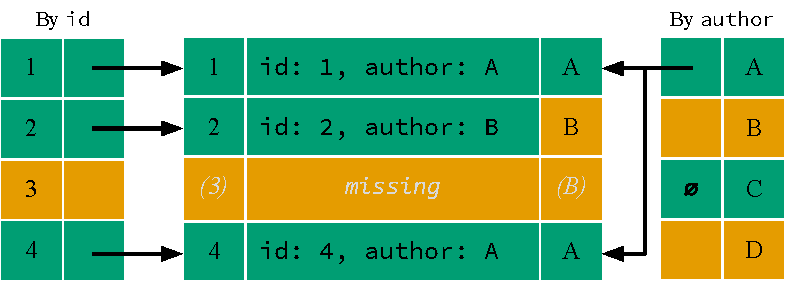
\includegraphics{diagrams/Indexing.pdf}
  \caption{Multiple indexes over the state in a single view in Noria. Even
  though \emph{some} rows for author B are present, some are missing and so the
  entry for B is considered missing in the \texttt{author} index. Even though no
  rows for author C are present, the index entry is not marked as missing, which
  would happen if Noria has checked that there are indeed no rows for
  author C.}
  \label{f:indexing}
\end{figure}

Missing state manifests as missing entries in particular indices. Indexes over a
given state are either all partial or none of them are. This may seem strange
based on how indices work in traditional relation databases.
Figure~\vref{f:indexing} gives an example with two different partial indices
over a view that holds a unique story identifier and the story's author. One
index is over the primary key column \texttt{id}, and one is over the story
author. Here, even though some rows with author B are present, the index entry
for author B is still considered missing, since not \emph{all} rows with author
B are present. This is necessary, as otherwise an application query for stories
authored by B would return an incomplete, and hence incorrect, result.
Similarly, while there are no rows for authors C or D, C is considered complete
because Noria has checked upstream that there are indeed no stories written by
C.

If, while processing an update, Noria encounters missing state, this indicates
that the update does not affect query results that the application has indicated
interest in. In such a case, Noria has two options: eagerly compute the missing
state before proceeding, or discard the update. To avoid unnecessarily
maintaining unimportant cached results, Noria drops updates in this case.

An important corollary of the above is that partial state must be enabled
on all stored state \emph{below} any partial state. It is illegal for the
dataflow to contain state for two nodes $A$ and $B$ where $A$ is an ancestor of
$B$, $A$ uses partial state, and $B$ does not use partial state. To see why,
consider what would happen if an update arrives at $A$ for a missing entry. $A$
would discard that update, and $B$'s state would remain perpetually stale.

\section{Upqueries}
\label{s:upqueries}

If an application requests data that is found to be missing, Noria issues an
\textit{upquery} to compute the requested data. Upqueries flow ``up'' the
dataflow graph, towards the base tables at the ``top'', and constitute a request
for the target of the upquery to replay past data. Upqueries may recurse if the
requested state is not available at the initial target.

The response to an upquery takes the form of a regular dataflow update that
flows down the dataflow. It combines all past deltas pertinent to the upquery
into a single update, and holds only positive deltas that represent the current
set of relevant records.

Operators are generally not aware whether they are processing an update that
resulted from a base table change or an upquery. The upquery response flows
in-line with other dataflow updates, and follows the edges of the dataflow.

Upquery responses are special in two key ways. First, they only propagate along
edges towards the operator that issued the upquery, so that one upquery does not
populate the relevant data in the state of \emph{every} operator. And second,
if an operator encounters missing state while processing an upquery response
update, it does not discard that update, but instead does the work necessary to
process that update. This process is described in further detail below.

When an application query encounters missing state in a view, Noria needs to
know what upqueries to issue. The set of necessary upqueries for each view is
that view's \textit{upquery plan}. Noria determines upquery plans by analyzing
each view's query when the application first installs that view, and deciding
how best to recompute its results. It does so by finding all \emph{possible}
upquery plans, choosing among them, and then informing all involved domains of
the chosen plan. There may be multiple possible candidates if there are multiple
equivalent ways to compute the missing state, such as by changing the direction
in which joins are executed as explained below.

\subsection{Key Provenance Tracing}

To determine what upqueries can be issued to reconstitute missing entries in a
given index, Noria must trace the view's parameter column back to a column in
upstream state. The intuition here is that in order to answer the application's
query of ``give me the results where column $C$ has value $x$'', Noria must be
able to replay rows where $C = x$ from somewhere. Or, phrased differently, when
the output for $C = x$ is missing, Noria must have a way to get at the inputs
that \emph{generate} $C = x$. As an example, if a view counts books by a given
author, and the current count for author $a$ is missing, Noria must be able to
somehow produce all books by author $a$.

\begin{figure}[t]
  \centering
  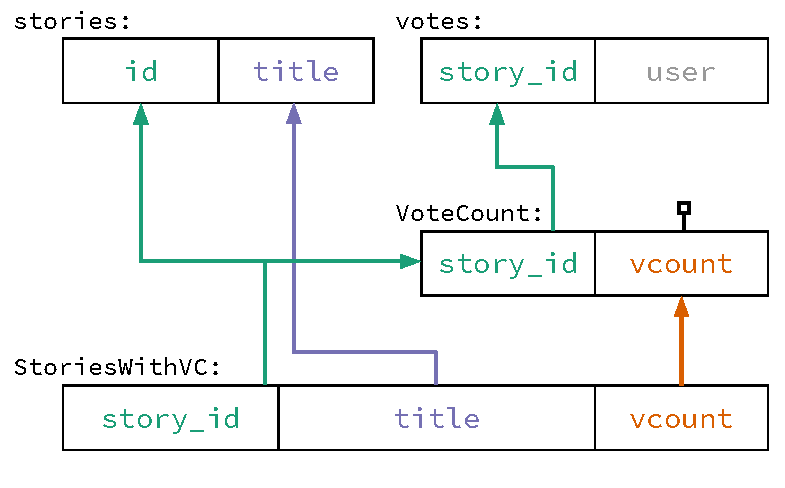
\includegraphics{diagrams/Key Provenance.pdf}
  \caption{Key provenance for each column in the \texttt{StoriesWithVC} view
  from Listing~\ref{l:vote-src}. Notice that \texttt{story\_id} has multiple
  base table origins, and \texttt{vcount} does not trace back to any base table
  columns. The query only uses \texttt{story\_id} as a parameter, so only its
  provenance is used to choose the upquery path.}
  \label{f:key-prov}
\end{figure}

More generally, in order to recompute the results where $C = x$ in some view
$V$, Noria must determine the \textit{key provenance} of $C$; where $C$ ``came
from''. Noria computes key provenance by tracing columns ``up'' the dataflow to
where they originate, which results in a provenance graph like the one shown in
Figure~\vref{f:key-prov} for the \texttt{StoriesWithVC} view from
Listing~\vref{l:vote-src}. The figure illustrates two important properties of
key tracing:

\begin{enumerate}
  \item An output column may trace to multiple input columns if it corresponds
    to the join column in a join, or if it passes through a union. The
    provenance of the \texttt{story\_id} column, for example, traces both to
    \texttt{stories.id} and \texttt{votes.story\_id}.
  \item An output column may be entirely computed, and thus have no association
    with a column in the inputs. The \texttt{vcount} column is computed by the
    \texttt{VoteCount} aggregation, and does not exist in the input data set.
\end{enumerate}

In Listing~\ref{l:vote-src}, Noria is asked to parameterize
\texttt{StoriesWithVC} by the \texttt{story\_id} column. The key provenance
graph tells Noria that it can request input data for a given \texttt{story\_id}
by sending an upquery either to the \texttt{stories} table using the \texttt{id}
column, or to the \texttt{vote} table using the \texttt{story\_id} column. Since
there exists a way to replay the input data for a missing output entry in this
case, the \texttt{StoriesWithVC} view can be made partial.

\paragraph{Broken Provenance.}
Consider what would happen if Listing~\ref{l:vote-src} had \texttt{WHERE vcount
= ?} as its parameter instead. If an application query misses in that case, the
upquery would have to be sent to \texttt{VoteCount}, and query for ``all stories
whose vote count is $x$''. If that state is present, all is well, but if
\texttt{VoteCount} is missing the state for \texttt{vcount = x}, there's a
problem. Noria now has no way to compute the missing state except by replaying
\emph{all} state in \texttt{vote} without an index. This would be equivalent to
a full table scan in a traditional database.
Noria's only%
%
\footnote{Noria cannot disable partial state just for \texttt{StoriesWithVC},
since that would violate place a partial index above a non-partial index, which
is illegal.}
%
efficient option is to disable partial
state for \texttt{VoteCount}. This ensures that any upquery to it never misses,
and therefore a table scan is never needed. Instead, the table scan is performed
only once: when the view is initially added. But this comes at the cost of
maintaining the entire resultset of the query for all parameter values.

\paragraph{Asymmetric Provenance.}
The join in Listing~\ref{l:vote-src} uses a inner join ($\bowtie$), and Noria is
therefore free to upquery \emph{either} side. If it upqueries the ``left'' side
of the join, the regular processing pipeline will perform the necessary lookups
into the ``right'' side of the join, and vice-versa. However, if the view query
used a left or right \emph{outer} join, Noria must upquery a particular side of
the join. For a left join, it must upquery the left ancestor, or risk missing
rows in the left ancestor that have no matching rows in the right ancestor. For
a right join, the same logic applies, but mirrored to the right ancestor.

\paragraph{Disjoint Provenance.}
If the provenance of a column crosses a union, \emph{all} ancestors of that
union must be upqueried, as opposed to just one as is the case with upqueries
through a join. Unlike with a join, the regular dataflow processing of the
upquery response through a union will not bring along results from the other
ancestors, so the requesting operator must ask them all individually.

\subsection{Path Selection}
\label{s:upquery:selection}

Once Noria has obtained a set of candidate upquery paths through key provenance,
it must decide on an upquery plan based on those paths. If there is only one
candidate, the choice is trivial. But with symmetric joins, multiple candidate
paths may be generated. Here, Noria is free to use whatever heuristics it sees
fit to decide which side of a symmetric join to send upqueries to. For example,
it may choose to send upqueries to the larger of the joined inputs so that fewer
lookups are necessary when processing the response.

In addition, key provenance tracing produces upquery paths that reach all the
way back to the origin of a column, which is usually located at the base tables.
However, it would be inefficient for operators to issue upqueries all the way to
the base tables on every miss. Some intermediate state may already have the
necessary data, and the upquery data could be sourced from there instead. Noria
therefore trims the paths from key provenance such that only the suffix of
operators starting at the last materialized state are included. For example, in
Figure~\ref{f:key-prov}, if Noria decides to upquery \texttt{StoriesWithVC}
through \texttt{VoteCount}, the upquery path would source its data from
\texttt{VoteCount}, not from \texttt{votes}.

If an upquery reaches its origin and finds that the requested state is missing
there too, a second upquery is issued using the origin's upquery paths, and only
when that upquery resolves does the original upquery resume. Upqueries may
recurse all the way up to the base tables this way, but avoid doing so if any
intermediate state can be re-used.

This process leaves Noria with a set of paths to upquery when it encounters a
missing entry in a given state.

\subsection{Implementing a Plan}

Once Noria has decided on a plan, that plan is communicated to all domains
that appear along each path in the plan. This is necessary so that each domain
knows where to route upquery responses that are part of a given plan, and does
not disseminate the response to the entire downstream dataflow.

When Noria announces the upquery plan, it may also add additional indices
to existing state to facilitate efficient execution of the new upqueries. In
particular, when an upquery arrives at the materialization it wants to source
data from, Noria needs an efficient way to find the requested data. Concretely,
Noria needs an index on the materialization whose key matches the lookup key of
the upquery. In this way, upquery plans adds additional indexing obligations
that Noria must take into account.

The key provenance information from Figure~\vref{f:key-prov} gives Noria all the
information it needs to set up these indexes: an index is needed on the upquery
key column on each state on the chosen upquery paths. In the case of the view
from Listing~\ref{l:vote-src}, an index is needed on
\texttt{StoriesWithVC.story\_id}, as well as either \texttt{stories.id} or both
\texttt{VoteCount.story\_id} and \texttt{votes.story\_id}\footnote{An index is
needed on \texttt{votes.story\_id} since the upquery to \texttt{VoteCount} may
recurse.}, depending on which upquery path Noria chooses across the join.

\section{Eviction}

Over time, the subset of data that the application cares about tends to change.
When it does, query results that were accessed previously may no longer be
important to maintain as they are no longer accessed. Partial state allows Noria
to cater to such changing application patterns by \textit{evicting} state
entries after they have been computed. When an entry is evicted, it is marked as
missing, and subsequent requests for that state trigger an upquery as usual for
missing state.

When Noria evicts an entry from state in the middle of the dataflow, the missing
entry may cause an update to be discarded even though downstream entries hold
data that would grow stale without that update. For example, consider what
happens if an operator counts the number of votes per author, and contains a
count of 7 for the author ``Jane''. Then, the state for ``Jane'' is evicted from
some operator upstream of the count. If an update now arrives at the operator
where ``Jane'' is missing; it would discard the update, and the downstream count
would remain perpetually stale.

To avoid such permanently stale entries, Noria must ensure that when an entry is
evicted, any dependent state downstream is also evicted. More formally, it must
ensure that:

\begin{invariant}
  \label{i:missing-suffix}
  If an operator encounters a missing state entry while processing a record $r$
  in an update, any downstream state that reflects $r$ must be evicted.
\end{invariant}

Upqueries as described thus far, without evictions, generally uphold this
invariant\footnote{Though not always; see \S\ref{join-evictions}}. As upqueries
recurse up the dataflow, missing state is filled in ``from the top down'' until
the operator that originally issued the upquery is presented with the requested
state. Any misses that occur during the processing of an upquery causes
recursive upqueries, which fill that missing state before proceeding.

To uphold the property in the face of evictions, Noria issues evictions
downstream whenever it decides to evict entries from state in the middle of the
graph. This ensures that any future update that touches the evicted state can
safely be discarded, as any relevant downstream state has been discarded as
well.

Invariant~\ref{i:missing-suffix} implies the corollary from earlier that partial
state cannot exist upstream of non-partial state. Since state cannot be evicted
from non-partial state, Noria would be unable to satisfy the invariant should it
ever encounter missing state upstream of the non-partial state.


\chapter{Practical Partial State}

The addition of partial state significantly changes how query results are
computed by the underlying dataflow system. This chapter demonstrates how
partial state is implemented in Noria such that it produces results similar to
those Noria would produce without partial state.

\section{Defining Correctness}

In order to discuss the degree to which partial achieves this goal, it is
necessary to first define what constitutes ``correct'' behavior, both in Noria
without partial, and with the introduction of partial.

\resume

\subsection{Correctness in Noria}

\subsection{Correctness with Partial State}

To give some intuition for why this problem is challenging, we first need to
understand what the goal of the system as a whole is. Ultimately, the partial
invariants all serve to maintain one principal property:

\begin{quote}
	If data stops flowing into the dataflow, the dataflow will eventually
	quiesce. When it does, for every key in every state, the value for that
	key is either missing, or it reflects the effects of each input to the
	system applied exactly once. A subsequent query for any missing key in
	any materialization populates the state for the missing key consistent
	with the property above for non-missing state.
\end{quote}

The intuition here is that Noria must \emph{at least} eventually do the right
thing. That is, it must make sure that all the data the application inserts into
the dataflow is considered, that none of it is double-counted, and that no other
spurious data is added. Unless, of course, the application has inserted dataflow
operators that double-count, in which case they should be exactly
double-counted.

We want Noria to provide stronger guarantees than eventual consistency whenever
possible and, in the common case, it does. Specifically, for most queries, Noria
ensures that a read from any given view sees complete query results as of some
recent time at each dataflow input. That is, for a given view, for each input
that feeds into that view, the view reflects a prefix of the data ingested by
that input. I call this \emph{prefix consistency}. Each view is also
continuously kept up to date; any new input is reflected in the view shortly
after being ingested, subject only to the propagation delay in the dataflow.

Noria does not necessarily provide prefix consistency when there are
\textbf{multiple} paths from a given dataflow input to a given view, such as
through a self-join. Depending on the precise semantics of the paths, this can
cause a view to briefly reflect \textbf{some} of the effects of newly inserted
data, but not all. For example, consider a self-join that computes a
parent-child relationship between records. If the application removes a record
$A$, that dataflow input must be processed along two edges. When it has been
processed by one edge, but no the other, the downstream view will briefly
continue to include $A$ as a child, even though it no longer appears as a
parent. This inconsistency is rectified once the dataflow input is also
processed on the second edge.

This problem is not directly related to partial state\,---\,Noria exhibits this
behavior when all state is fully materialized. However, partial state must work
in the context of such temporary inconsistencies. Furthermore, partial state
should not exaggerate these problems by introducing additional inconsistencies.

There are several situations that arise in a real dataflow implementation that
make even this seemingly simple property difficult to uphold. I sketch the
primary ones below, and give brief descriptions of my proposed solutions. In my
thesis, I will go into these in greater detail. I will also provide a more
comprehensive analysis of the possible inconsistencies that can arise if these
situations are not handled correctly by the partial state logic.

At its core, partial state introduces two new conditions into the dataflow that
were not previously present. First, multiple updates may now be collapsed and
re-processed through the dataflow as a single, consolidated update in response
to an upquery. These consolidated updates represent \textit{snapshots} of
upstream state, and the system must ensure that these snapshots do not introduce
duplicate or spurious query results, or fail to include relevant data.

Second, with partial state in place, \emph{any} operator processing may
encounter missing state. When that happens, the system

\section{Linear Dataflow}

First, consider a single strand of dataflow, where each operator has at most one
input and at most one output. For partial state to be correct, it must be the
case that computing missing results with an upquery that combines all past
deltas into a single update produces the same results as processing the deltas
one-at-a-time.

\begin{inprogress}
  What about discarded updates in the paragraph below?
\end{inprogress}

The deltas that flow through the dataflow system represent changes to the
logical output state of the operator that produced the delta. If a base table
produces a negative delta for a row $r$, it means that row $r$ is no longer part
of that base table's current state. An upquery fetches current state, which is
the sum of all past deltas emitted by the queried operator, and then feeds it
through the same chain of dataflow operators that individual deltas go through.
For upquery processing to be equivalent to one-at-a-time delta processing, it
must be the case that with operators $f_1$ through $f_N$, and past deltas $d_1$
through $d_M$:

\begin{eqnarray*}
  \sum^M_{i=1}\left(f_N \circ \dots \circ f_1\right)\left(d_i\right) = \
  \left(f_N \circ \dots \circ f_1\right)\left(\sum^M_{i=1}d_i\right)
\end{eqnarray*}

With a single operator, this trivially holds since all Noria operators are
distributive over delta addition:

\begin{eqnarray*}
  \sum^M_{i=1}f\left(d_i\right) = \
  f\left(\sum^M_{i=1}d_i\right)
\end{eqnarray*}

Using this property, it is possible to ``shift'' the delta sum across operator
compositions:

\begin{eqnarray*}
  \sum^M_{i=1}\left(f_{n+1} \circ f_n\right)\left(d_i\right) &=& \sum^M_{i=1}f_{n+1}\left(f_n\left(d_i\right)\right) \\
  &=& f_{n+1}\left(\sum^M_{i=1}f_n\left(d_i\right)\right) \\
  &=& f_{n+1}\left(f_n\left(\sum^M_{i=1}d_i\right)\right) \\
  &=& \left(f_{n+1} \circ f_n\right)\left(\sum^M_{i=1}d_i\right)
\end{eqnarray*}

Therefore, the same ultimate state results whether the system executes each
dataflow operator in sequence on individual deltas, or whether it first sums
all the deltas into a single update, and then executes the operators in sequence
over that. Or, stated differently, if normal dataflow processing produces the
correct result, so too must processing a combined upquery response.

\section{Diverging Dataflow}

Dataflow graphs for real applications are rarely linear. They contain branches
where the dataflow diverges, such as if two views both contain data from the
same table.

\resume

\section{Merging Dataflow}

In practice, most applications include at least one join or union in their
queries. When they do, strands of dataflow combine to produce joint output that
depends on both inputs. And crucially, such dataflow constructions introduce the
possibility of data races. Now, updates may be arriving to an operator from two
inputs in parallel, and the operator may process either update before the other.
Furthermore, upqueries must now retrieve data from \emph{all} ancestors, and
ensure that they are combined in such a way that no duplicate or spurious data
is introduced, and no data is missed.

\resume

Operators that have multiple ancestors pose a problem to the partial
model. Consider an identity operator that merely combines the input
streams of its ancestors (i.e., a union). An upquery that crosses this
operator must \emph{split} its upquery; it must query each ancestor of the
operator, and take the union of the responses to populate missing state.
But when we allow concurrent processing, these responses may be
arbitrarily delayed between the different upquery paths.

Let's examine what happens with a union, U, across two inputs, A and B,
and a single materialized and partial downstream operator C. C discovers
that it needs the state for $k = 1$, and sends an upquery for $k = 1$ to
both A and B. A responds first, and C receives that response. It needs
to remember that the missing state is still missing, so that it does not
expose incomplete state downstream (e.g., if it received an upquery for
$k = 1$, it could not reply with \textbf{just} A's state). Now imagine that
both A and B send one normal dataflow message each, and that they both
include data for $k = 1$. When these messages reach C, C faces a
dilemma. It cannot drop the messages, since the message from A includes
data that was not included in A's upquery response. If it dropped them,
that data would disappear forever, which violates our primary system
property. But it also cannot apply the messages, since B's message
includes data that will be included in B's eventual upquery response. If
it did, that data would be duplicated.

How upqueries work across multi-ancestor operators depends on the
semantics of that operator. For unions, as we saw above, the upquery
must go to all the ancestors. For joins on the other hand, the upquery
must only go to \textbf{one} ancestor. This is because when a join processes
a message from one ancestor, it already queries the ``other'' ancestor and
thus pulls in any relevant state. In the example above, if U were a
join, then if C sent an upquery to both A and B, the two upquery
responses it received would contain duplicate data. For a symmetric
join, the responses would in fact be identical, whereas for an
asymmetric join (like a left join), they would differ. This suggests
that we must determine the algorithm for upqueries across each type of
multi-ancestor operator separately. Unions, joins, and left joins for
example all have different upquery restrictions.

\subsection{Unions}

Unions must buffer upquery results until all their inputs have responded. In the
meantime, they must buffer updates for the buffer upquery keys to ensure that a
single, complete, upquery response is emitted.

\subsection{Congruent Joins}

Joins already contain implied upqueries, so only one side must be upqueried,
with the upqueries to the other side left to the join itself. Left joins work
the same way, but with the additional restriction that the initial upquery
\emph{must} go the left input.

Sometimes, an operator must issue an upquery upstream in order to
satisfy an upquery from downstream. I refer to a recursive upquery like
this as a \emph{dependent} upquery. Dependent upqueries are not, in and of
themselves, complicated. They function exactly like a regular upquery.
However, it turns out they pose a challenging system design problem.

Upquery responses must, in some sense, be atomic. They must occur at
some single logical point in time with respect to an operator's input
and output streams. Consider what happens if an operator is part-way
through processing an upquery response, and discovers that it must
perform a dependent upquery in order to complete that processing. It may
be a while before the dependent upquery resolves, and in the meantime
the operator needs to decide what to do.

If it blocks waiting for the response to come back, it holds up all
processing of other upqueries and writes. That would not be great. On
the other hand, if it continues processing other inputs, it risks
dropping or duplicating inputs; any part of the upquery response it
produced \textbf{before} it found the need for the dependent query still
reflects the state at that point in time. Since it may have processed
writes since then that affect that computed state, the upquery response
would no longer reflect a current, atomic snapshot.

\paragraph{Noria solution}
Operators issue dependent upqueries only if the need arises while processing an
upquery response. Otherwise, that part of the current update is discarded. If a
dependent upquery must be issued to complete processing some past upquery
response, the response is dropped, the dependent upquery is issued, and the
operator re-tries the original upquery when the dependent upquery resolves.

\begin{inprogress}
  Should also mention self-lookups on different columns (are there any?).
\end{inprogress}

\subsection{Incongruent Joins}

We have to guarantee that all data relevant to a given state entry
eventually reaches that state. A corollary of this is that we cannot
discard messages that may affect non-missing, downstream state.
Normally, this is the case, since upqueries traverse the dataflow from
the leaves and ``up''\,---\,if some key $k$ is present at an edge down the
graph, it is also present at every materialization above that edge, and
therefore messages with key $k$ will not be discarded early.

Unfortunately, this only holds for upqueries where all dependent
upqueries share the same key as the leaf-most upquery. Consider a
dataflow that joins two inputs, \texttt{Article} and \texttt{User}, on the article's
author field. A downstream operator then issues an upquery for article
number 7. The upquery is issued to \texttt{Article}, which produces a message
that contains article number 7 with, say, author ``Elena''. That message
arrives at the join, which issues a dependent upquery to \texttt{User} for
``Elena''. When that dependent upquery resolves, the join produces the
final upquery response, and the state for article number 7 is populated
in the downstream materialization.

Next, an editor changes the author for article number 7 to ``Talia''. This
takes the form of a message with a negative for \texttt{[7, "Elena"]} and a
positive for \texttt{[7, "Talia"]}. When this message arrives at the join, it
may miss when performing the lookup for ``Talia''. The join therefore
drops \texttt{[7, "Talia"]}, and only the negative for ``Elena'' propagates to
the downstream materialization. It then marks the state for article
number 7 as empty (though not missing). Any subsequent read for article
number 7 receives an empty response, which violates our primary system
property.

\paragraph{Noria solution}
Key provenance analysis detects when the dataflow downstream of an operator has
this property. With that information, an operator knows when it is about to drop
an update that \emph{may} nonetheless exist in downstream state. It issues an
eviction for that state, ensuring that if the updated state is subsequently
needed, it will be queried for.

\section{Diamonds}

\section{Sharding}

Noria supports sharding cliques of operators to increase the throughput
of particular sections of the dataflow. Shards of an operator execute in
parallel, without synchronization. Edges that cross from an unsharded
operator to a sharded one split its outgoing updates using hash
partitioning. Edges that cross back have an implicit union injected to
merge the sharded results. Edges that cross from one sharding to a
different sharding are merged and then split again. Upqueries must also
work when Noria decides to shard operators in this way.

Upqueries across a sharding boundary are a complicated affair. The
operator that issues the upquery must determine which shard or shards to
send the upquery to. If it queries multiple shards, the responses from
those shards are subject to the same multi-ancestor issue as unions.
When a response to the upquery comes back, it must be specifically
routed to only the requesting shard, so that it does not accidentally
populate the state of other shards. This logic must work even if
multiple shards issue an upquery for the same key concurrently. Or,
worse yet, if a single upquery must traverse \textbf{multiple} sharding
boundaries.

\paragraph{Noria solution}
Key provenance informs operators whether an upquery for a given column should be
sent to all shards, or just one shard, of the upquery source. This information,
as well as the shard identifier of the requesting operator, is included in the
upquery itself, and in the eventual response. Sharding unions buffer upquery
responses that originated from more than one shard (like regular unions). Shard
``splitters'' ensure that responses only arrive at the requesting shard using
the requestor information in the response.

\section{Miscellaneous Lifted Text}

\begin{inprogress}
  Nothing should remain in this section.
\end{inprogress}

\subsection{Consistency}

How do we know that Noria is eventually consistent?

First, how do we know that Noria without partial state is eventually
consistent. And second, how do we know that Noria remains eventually
consistent with partial state.

We don't have a formal proof for either. Ignoring implementation bugs, the
informal argument goes something like:

For partial state, we need to show that each of the things that have been
changed preserve eventual consistency. First, sending a snapshot of past state
(upquery response) is equivalent to sending the individual updates that made
up that snapshot since the operators are distributive and commutative. Second,
upquery results can race with related updates, which is handled by the various
challenges I listed in the proposal:

 - sending them inline in the dataflow (for single-branch)
 - union buffering (for unioned branched dataflow)
 - special join upquery handling (for joined branched dataflow)

And third, partial state means that lookups can miss internally in the
dataflow, which is handled by join eviction when related state may still be
present downstream, and by discarding the update when it is not.


\chapter{Evaluation}

This thesis is built on the belief that view materialization is useful, but
prohibitively costly to use with current solutions. It presents partial state as
a solution to this problem that allows retaining the benefits of view
materialization at a fraction of the cost. Section \ref{s:eval:why} evaluates
the validity of this assumption, and the efficacy of partial state as a
solution.

Existing application deployments tend to implement their own ad-hoc caching
logic, usually by placing a dedicated cache in front of the database. Some
larger companies have also built comprehensive tooling to manage their caches
correctly. Section \ref{s:eval:alts} looks at how Noria serves as an attractive
alternative to these approaches.

With partial state, only a subset of each view is materialized, and missing
results are computed on-demand. Partial state thus presents a trade-off between
memory use (cache size) and tail latency (miss rate). Section \ref{s:eval:cost}
explores the effects of this trade-off.

Developers may be hesitant to switch applications that already use a cache today
to Noria without some evidence that their performance won't regress.
Unfortunately, the impact Noria would have on any given application is highly
dependent on the particulars of each application, and is thus hard to measure.
To demonstrate that Noria can offer comparable absolute performance to existing
caching solutions, section \ref{s:eval:kvperf} compares Noria lookup performance
to that of Redis under ideal caching conditions.

An added benefit of partial state is that it allows applications to introduce
new queries/views without materializing it entirely up-front. This enables fast
adoption of new queries, but also means that queries to new views are initially
slow. Section \ref{s:eval:mig} evaluates these partial state migrations compared
to traditional all-at-once materialization.

The ability of partial state to reduce the memory use of view materialization
depends on skew in the application's data and access patterns. It allows Noria
to reduce latency for a significant fraction of requests by keeping only a few
results cached. While it is impossible to predict the skew for an arbitrary
application's data and queries, section \ref{s:eval:patterns} gives a simplified
theoretical model to help with estimation.

\section{Experimental Setup}
\label{s:eval:setup}

The experiments in this chapter primarily use the Lobsters news
aggregator web application at \url{https://lobste.rs}~\cite{lobsters}. This
application was chosen because it is open-source (so we can see what queries it
issues), because it resembles many larger-scale applications (like Hacker News
or Reddit), and because statistics about the site's data and access patterns are
available~\cite{lobsters-data}.

The evaluation uses a workload generator that issues page requests
according to the available statistics~\cite{generator}. It does not run the
real Lobsters Ruby-on-Rails application, as it is prohibitively slow. Instead,
all experiments use an adapter that turns page requests directly into the
queries the real Lobsters code would issue for that same page request. The
generator supports scaling up the rate of access and user count to emulate a
larger user base for benchmarking.

\begin{figure}
  \begin{tabular}{ p{0.8in} | r | r | r | p{2.9in} }
    Page & \% & W & Q & Description \\
    \hline
    Story & 55.8 & 1 & 14 & Renders an individual story's page, including its
    popularity score, comments, and the scores of its comments.\\
    Frontpage & 30.1 & 0 & 14 & Lists the 25 most highly scored stories, along
    with their authors and scores.\\
    User & 6.7 & 0 & 7 & Renders a user summary page, including what story
    ``tags'' they contribute to.\\
    Comments & 4.7 & 0 & 9 & Like the frontpage, but for comments.\\
    Recent & 1.0 & 0 & 14 & 25 most recently added stories, along with their
    authors and scores.\\
    Vote & 1.2 & 1 & 2 & Vote up/down a given comment or story.\\
    Comment & 0.4 & 2 & 5 & Add a new comment to a story.\\
  \end{tabular}
  \caption{Pages in Lobsters. \% indicates the percentage of requests that load
  the given page. W is the number of writes loading the page requires, and Q is
  the number of queries it issues.}
  \label{t:lobsters-pages}
\end{figure}

The various pages in Lobsters differ significantly in what queries they issue,
how many queries they issue, and the extent to which they are read or write
heavy. Table~\ref{t:lobsters-pages} gives an overview of the frequency of
requests for each page, what loading the page entails, and a brief description
of that page. In all evaluation results, latency is measured across all
requests, no matter what page they are for.

Experiments run on Amazon EC2 r5n.4xlarge instances, which have 16 vCPUs and
128GB of memory. The server is always given a dedicated host, while
load-generating clients are split across one or more m5n.4xlarge instances
depending on the desired load factor.

The benchmarks are all ``partially open-loop''~\cite{frank-open-loop}:
clients generate load according to a workload-dictated distribution of
interarrival-times, and has a limited number of backend requests outstanding,
queueing additional requests. This ensures that clients maintain the measurement
frequency even during periods of high latency. The test harness measures offered
request throughput and ``sojourn time''~\cite{open-loop-cautionary-tale}, which
is the delay the client experiences from request generation until a response
returns from the backend.

All experiments measure memory use using the resident virtual memory of the
server process (VmRSS). This measurement therefore includes all indexes, runtime
allocations, and other bookkeeping metadata. For Noria, it also includes the
data stored in the base tables.

Since the benchmarks introduce more data as they run, memory use increases over
the course of each run. Experiments are run for a bit over 5 minutes unless
otherwise specified, and memory measurements are taken at the end of the run.

\begin{inprogress}
  Note about stability of experimental results once all experiments are nailed
  down.
\end{inprogress}

\section{Benefits and Costs of View Materialization}
\label{s:eval:why}

The core argument of this thesis is that partial state makes view
materialization feasible. Bundled up in that argument are several intertwined
questions that must be answered before further evaluation of partial state is
interesting:

\begin{enumerate}
    \item Why is view materialization desirable?
    \item Why is view materialization not feasible currently?
    \item Does partial state improve on this situation?
\end{enumerate}

\begin{figure}[h]
  \centering
  \includegraphics{graphs/lobsters-throughput.pdf}
  \caption{Maximum achieved throughput on Lobsters benchmark with and without
  view materialization. Without view materialization, MySQL must compute query
  results each time. Traditional (full) view materialization runs out of memory
  at $\approx$4.6k pages/second. Partial state allows Noria to reduce memory use
  significantly so that it can achieve higher throughput.}
  \label{f:lobsters-throughput}
\end{figure}

Figure~\ref{f:lobsters-throughput} attempts to explain why view materialization
is desirable. It compares the highest sustainable request load of three
different systems: MySQL, Noria without partial state, and Noria with partial
state. MySQL is run entirely in RAM by running it on a ramdisk, and on its
lowest isolation level. The figure shows the highest Lobsters throughput each
system achieves before its mean latency exceeds 50ms.

View materialization alone (as provided by Noria) improves performance by almost
$12\times$ compared to MySQL, as query results are now frequently cached.
However, without partial state, this performance increase comes at a significant
memory cost. Beyond 4.6k pages/second, it runs out of memory, and cannot
support the workload. With partial state, Noria uses much less memory at a given
load factor, which allows it to support 67\% higher throughput, almost
20$\times$ that of MySQL%
\footnote{The Noria benchmarks are memory constrained, not CPU constrained.
MySQL fully loads all 16 cores at 391 pages per second.}.

\begin{figure}[h]
  \centering
  \includegraphics{graphs/lobsters-memory.pdf}
  \caption{Memory use two minutes into the Lobsters benchmark at 4.6k pages per
  second. Striped bars store base tables on disk using RocksDB.}
  \label{f:lobsters-memory}
\end{figure}

Figure~\ref{f:lobsters-memory} shows the memory use at 4.6k pages per second
with and without partial state. It demonstrates both the issues with full
materialization, and the improvements brought about by partial state. With full
materialization, Noria must store every result for every query in memory. In
contrast, with partial state, Noria stores only frequently accessed results,
which cuts memory use in half.

The memory use reductions with partial state are a direct result of the skew in
Lobsters data popularity and access patterns. Many pages are simply never
visited over the course of the benchmark, and so need not be brought into the
cache. With partial state, Noria also evicts infrequently accessed results,
which further reduces memory use, and ensures that the cache does not eventually
grow to contain all results.

\begin{figure}[h]
  \centering
  \includegraphics{graphs/lobsters-opmem.pdf}
  \caption{Estimated operator state data size two minutes into the Lobsters
  benchmark at 4.6k pages per second. The value indicated includes only the sum
  total size of rows in each operator's state, not data structure overheads,
  indices over the data, or other memory allocations. Base tables are not
  included.}
  \label{f:lobsters-opmem}
\end{figure}

Much of Noria's memory use goes to storing the base tables in memory. Since
partial state cannot evict base table state, this limits how much memory can
potentially be saved. The figure therefore also includes memory use when running
Noria with its durable RocksDB storage backend for base tables. In that
configuration, base tables are kept on disk, not in memory, which makes the
memory savings from partial state more apparent\,---\,the memory use is now
about a third that without partial state.

Various other runtime overheads that partial state cannot eliminate remain, such
as data structure overheads, and allocations for in-flight requests and pending
responses. With diligent memory optimization, this overhead could likely be
further reduced to increase the relative benefits from partial state. To provide
some insight into how far memory use can be reduced,
Figure~\ref{f:lobsters-opmem} shows the total size of the data contained in all
non-base operator state in Lobsters. This metric measures \emph{only} the sum of
the data in each row, and excludes all other memory overheads, such as hash
tables, additional indices, or allocations elsewhere in the application. The
results indicate that partial state in isolation requires only 1.5\% of the
total operator state to be materialized; significantly less than the
$\sfrac{1}{3}$ seen in Figure~\ref{f:lobsters-memory}. This suggests that there
is further potential for reducing partial state's memory footprint.

Since partial state uses less memory, applications that do not need higher
throughput can instead reduce cost by using hosts with less memory. For example,
on AWS EC2, going from a 64GB instance type with 16 cores (\texttt{m5n.4xlarge})
to a 128GB instance type with 16 cores (\texttt{r5n.4xlarge}) comes at a 25\%
price increase. Instances with 256GB of memory only come with 32 cores
(\texttt{r5n.8xlarge}) or more, and come out at twice the price of 128GB.

\section{Rolling Your Own}
\label{s:eval:alts}

Many applications already require lower latency and higher throughput than
straightforward SQL queries against traditional relational databases provide.
Developers often implement manual optimizations to improve their application
performance, and introduce additional complexity into their applications in the
process. These optimizations usually come in one of two forms: denormalization
and caching. This section discusses each of these optimization techniques in
turn, as well as how Noria makes them unnecessary.

\subsection{Denormalization}

The relational database model~\cite{relational} encourages developers to use
``normalized'' schema in which redundant data%
\footnote{The relational model differentiates between strongly and weakly
redundant data\,---\,``redundant'' here refers to strong redundancy.}
that can be derived from other data is not stored. Instead, the model suggests
that derived or computed data be produced on-demand using relational operators
like joins and aggregations. The original paper then adds:

\begin{quote}
Only in an environment with a heavy load of queries relative to other kinds
of interaction with the data bank would strong redundancy be justified in the
stored set of relations.
\end{quote}

As discussed in the motivation section for this thesis, many web applications
fall into exactly this category. Queries are far more common than inserts or
updates, and with a normalized schema they must constantly expend resources to
re-compute such derived data. For this reason, web developers often explicitly
denormalize their schema to include data that would be prohibitively expensive
to compute on-demand.

For example, in Lobsters, each story has a ``hotness'': a score of how popular a
story is, and thus how far up it should appear in listings. This value depends
on a lot of parameters, such as the number of votes, the number of comments,
etc. It would be prohibitively expensive to compute a story's hotness directly
in the queries, especially in the context of computing the front page view,
which requires the hotness for \emph{all} stories to rank them. Instead, the
Lobsters developers add a computed column, \texttt{hotness}, to the
\texttt{story} table. This column is then updated whenever relevant data
changes, such as when:

\begin{itemize}
    \item a story is upvoted or downvoted.
    \item a comment is added to a story.
    \item a comment on a story is upvoted or downvoted.
    \item a comment or vote is deleted.
    \item one story is merged into another.
\end{itemize}

There are several such computed columns in Lobsters. For each one, developers
must inspect all write paths, and change them to ensure that they correctly
update all related computed values. This process is manual and error-prone, but
also necessary: without these manual optimizations, Lobsters running against
MySQL cannot keep up with even a single request per second.

With Noria, such manual denormalization is unnecessary. View materialization
automatically stores and maintains derived data so that it is efficient to
query. The developer can continue to use normalized schemas and queries, and
does not need to modify their application code to manage denormalized columns
and tables.

\subsection{Caching}

If denormalization does not sufficiently improve the application's performance,
the next step is usually to add a cache in front of the database. This cache
often takes the form of a key-value store, like Redis or Memcache, which holds
frequently accessed, computed results. When the application issues a query, it
checks the (fast) cache first, and only if the results are not available in
cache is the (slower) backend consulted.

A dedicated cache speeds up reads that hit, but introduces significant
application complexity. Just like for manual denormalization, all parts of the
application that modify data related to any given cache entry must know to also
invalidate or update the cache. In addition, the developers must ensure
that if multiple clients miss on a given entry, they do not hit the backend
database all at once. This is especially important if a popular entry is
invalidated, as it may cause a ``thundering herd'' effect where a large number
of clients swarm the backend and overwhelm it. Furthermore, since the clients
must now access two separate systems, mechanisms must be in place to ensure that
the cache remains consistent with the underlying data. This is difficult since
data may be updated at any time, including just after a client has fetched the
(then) latest data from the database to update the cache.

Because of the challenges above, implementing caching ``correctly'' requires
highly sophisticated machinery~\cite{facebook-memcache, transactional-cache,
orm-cache, sql-cache}, which developers may not even think to employ. A survey
from 2016 found that 0.3-3.0\% of application code spread across 2.1-10.8\% of
the application's source files is caching-related, and that cache-related issues
make up 1-5\% of all issues~\cite{caching-is-hard}.

With Noria, there is no need to maintain such a query result cache, as Noria's
in-memory materialized views provide high-throughput, low-latency queries
directly from the database. Thanks to partial state, Noria's materialized views
are usable even for applications whose full cache state exceeds the amount of
memory available on the server host. Since Noria automatically maintains the
materialized views, the application also does not need code to manage cache
invalidation or to address challenges like thundering herds.

\section{The Memory/Latency Trade-off}
\label{s:eval:cost}

Partial state's main drawback compared to complete materialized views is
that the results for an application's query may not be known. Or, stated
differently, some reads may miss. When this happens, the system must upquery the
missing state, which takes time and consumes resources otherwise dedicated to
writes. This shows up as increased tail latency for the application: queries
whose results are not known must wait to be computed. The hope with partial
state is that, once the commonly-accessed query results are cached, latency
quickly drops such that going forward only infrequently accessed query results
must be computed on-demand.

\subsection{Warming the Cache}

\begin{figure}[t]
  \centering
  \includegraphics{graphs/lobsters-timeline.pdf}
  \caption{Lobsters latency timeline at 1.5k pages per second across all pages
  with eviction. Figure shows the latency profile seen by the client over time,
  starting at the point when the first query is issued. Time increases along the
  x-axis, with each bin sampling twice as long as the previous one. The measured
  latency for each time bin is plotted on a logarithmic scale on the y-axis.
  Progressively lighter colors include more of the tail.}
  \label{f:lobsters-timeline}
\end{figure}

The cost of these misses is particularly visible when Noria starts with empty
state. This is equivalent to starting a more traditional caching system with an
empty (cold) cache, and having to ``warm'' it by filling in the most popular
entries. To measure this warming period, Figure~\ref{f:lobsters-timeline} shows
the latency profile seen by the Lobsters benchmark described in
\S\ref{s:eval:setup} over time, starting at the point when the first query is
issued. Time increases along the x-axis, and the measured latency for each time
bin is plotted on a logarithmic scale on the y-axis. Progressively lighter
colors indicate values further into the tail.

The figure shows that latency is initially high, but after a few seconds, the
mean and 95th percentile latency drop below 10 milliseconds. By the time a
minute has passed, the 99th percentile has followed suit. Since only a small
portion of the total computed state is cached (as shown in
Figure~\ref{f:lobsters-memory}), this supports the hypothesis that partial state
achieves low latency once the most commonly accessed results are cached.
The latency is primarily determined by the number of queries each page issues,
as each one requires a round-trip to Noria.

\subsection{Impact on Tail Latency}

\begin{figure}[h]
  \centering
  \includegraphics{graphs/lobsters-memlimit-cdf.pdf}
  \caption{CDF of sojourn latency across all Lobsters pages at 1.5k pages per
  second with decreasing permitted memory use. The figure depicts steady-state
  operation\,---\,the benchmark has been allowed to run for two minutes before
  the latency is measured.}
  \label{f:lobsters-mem-latency}
\end{figure}

Partial's trade-off is that of memory use versus tail latency; as you allocate
less memory to Noria, less of your tail can be pre-computed, and thus more of
your requests will be slow as it must be computed on-demand.
Figure~\ref{f:lobsters-mem-latency} shows this trade-off in the steady state%
\footnote{The benchmark runs for two minutes before latencies are sampled.}
of the application. It plots the CDF of the sojourn latency across all requests
with increasingly aggressive eviction. As Noria is asked to
reduce memory use by evicting more aggressively (darker purple lines), more
requests take longer, and the tail grows. In other words, the further you want
to reduce memory use, the more you pay in latency. Without partial
materialization, you do not have this choice\,---\,requests in the tail will
always be fast, but only as long as all the materialized views fit in memory.

\begin{figure}[h]
  \centering
  \includegraphics{graphs/lobsters-durability-cdf.pdf}
  \caption{CDF of sojourn latency across all Lobsters pages at 1.5k pages per
  second with base tables in memory and on disk. The figure depicts steady-state
  operation\,---\,the benchmark has been allowed to run for two minutes before
  the latency is measured.}
  \label{f:lobsters-dur-latency}
\end{figure}

If base tables are not kept in memory, the cost of recomputing missing state
from the data in those base tables increases. Exactly how much depends on the
performance characteristics of the durability backend in use.
Figure~\ref{f:lobsters-dur-latency} shows a CDF of page latencies when Noria's
RocksDB backend is used, with writes going to a ramdisk. Latencies increase by
anywhere from 20-50\%, depending on the number of misses a given page request
experiences.

The reason why the whole curve shifts, rather than just the tail, is that these
CDFs are across \emph{all} the different page types in Lobsters. Each one issues
a different set of queries, and so their total time differs, as does the effect
of a longer tail. The exact shape of this curve, and how it shifts in response
to varying resources, depends on the application in question.

% \begin{inprogress}
% Full materialization is slightly faster than partial materialization because
% SOMETHING SOMETHING either join eviction or faster lookups due to no tombstones?
% \end{inprogress}

\subsection{Memory Use and Throughput}

Memory use can only be reduced so far before the system no longer keeps up with
the offered load. If some of the most frequently accessed (``hot'') query
results are not cached, the system will constantly have to re-compute those
results to satisfy reads that come in shortly after that query result is
evicted. This cache churn increases latency and decreases throughput, often
significantly. Essentially, the system will never finish warming the cache, and
latency will remain at the high levels shown early in
Figure~\ref{f:lobsters-timeline}. For Lobsters, this happens around the 18GB
mark. If the eviction is tuned to be more aggressive than that, Noria can no
longer sustain 1.5k pages per second.

Generally speaking, as throughput increases, so must the memory budget. The
intuition behind this is that the memory budget effectively dictates your hit
rate. The more requests are issued per second, the more misses (in absolute
terms) result from a given hit rate. If those misses in the tail are
distinct, Noria must satisfy \textbf{more} upqueries as load increases, while
also handling that added load.

\begin{listing}[h]
  \begin{minted}{sql}
    SELECT articles.*, COUNT(votes.user_id)
    FROM articles
    LEFT JOIN votes ON (articles.id = votes.article_id)
    GROUP BY articles.id
    WHERE articles.id = ?
  \end{minted}
  \caption{Simplified query for vote counting in Lobsters.}
  \label{l:votes}
\end{listing}

While this correlation between throughput and memory use exists in Lobsters, it
is difficult to show clearly as each page issues many different queries, and
overall load is relatively low. For this reason, the next set of benchmarks use
a simplified version of one particular query from Lobsters shown in
Listing~\ref{l:votes}. It counts the number of votes for an article, and
presents that alongside the article information. The benchmark issues requests
distributed as 99\% reads and 1\% writes (inserts into \texttt{votes}). The
access pattern is skewed such that 90\% of requests access 1\% of keys across
10M articles%
\footnote{The benchmark samples keys from a Zipfian distribution with a skew
factor ($\alpha$) of 1.15}. Load is generated by four clients, and each one
batches requests for a maximum of 10ms to reduce serialization overheads.

\begin{figure}[h]
  \centering
  \includegraphics{graphs/vote-throughput-memlimit.pdf}
  \caption{Achieved throughput vs 95th percentile request latency in vote with
  increasingly aggressive eviction. Offered load increases along the points on
  each line. A near-vertical line indicates that the system no longer keeps up
  with offered load.}
  \label{f:vote-throughput-memlimit}
\end{figure}

Figure~\ref{f:vote-throughput-memlimit} demonstrates the connection between
throughput and memory use. It shows throughput-latency lines for the vote
benchmark with progressively more aggressive eviction. Each point along each
line is a higher offered load; its x-coordinate is the achieved throughput, and
its y-coordinate is the measured median latency. When Noria no longer keeps up,
you see a ``hockey stick'' effect, where achieved throughput no longer
increases, while latency spikes.

The figure shows that as the offered load increases, Noria needs to use more
memory to keep up. If we do not bound memory use, Noria can keep up with higher
load at the cost of caching most of the dataset (about two thirds).

\section{Absolute Cache Performance}
\label{s:eval:kvperf}

Despite how error-prone the approach is, ad-hoc, per-application caching is
still common in practice. And while Noria eliminates most of the developer
burden of getting caching right, it must offer competitive performance with
manually constructed caching solutions to present a viable alternative.

Unfortunately, this is difficult to evaluate, since high-performance solutions
are often developed specifically for a given application, and not available as
general-purpose tools. And effectively applying the general-purpose tools that
\textbf{are} available, like memcache and Redis, requires significant effort on
the part of the application authors (or the evaluators). To manually add caching
support to Lobsters' ~80 queries, including thundering herd mitigation and
incremental updates, would be a significant undertaking.

This fact alone is, in essence, an argument for the Noria approach. The manual
effort involved in making Lobsters use Noria is minimal\,---\,just switch the
code to query Noria instead of MySQL, and you get automatic caching. In many
cases the application code can even be simplified, such as by removing manual
materialization decisions like the story ``hotness'' column described in
\S\ref{s:eval:alts}.

Nevertheless, an experiment to evaluate Noria's absolute performance compared to
a ``real'' cache is necessary. Without such a comparison, Noria can only claim
to be ``faster than MySQL'', but not ``as fast as a cache''.

The next experiment runs the vote benchmark from Listing~\ref{l:votes} against
Redis~\cite{redis}, a popular high-performance key-value store that is commonly
used as a caching backend. In an attempt to approximate how a carefully planned
and optimized application caching deployment might perform, it makes the
following modifications to the benchmark:

\begin{itemize}
 \item Every access hits in cache, to emulate perfect thundering herd mitigation
   and invalidation-avoidance schemes.
 \item Nearly all accesses (99.99\%) are reads, since writes would be
   bottlenecked by the backing store.
 \item Data is not stored anywhere except Redis.
 \item Accesses are batched to reduce serialization cost and increase
   throughput. Specifically, reads are \texttt{MGET}s, and writes are pipelined
    \texttt{INCRBY}s.
\end{itemize}

This is not a realistic use of Redis as a cache, and ignores the complexities of
integrating the cache with the application. It also assumes that cached query
results are never spread across more than one key in the cache. However, it
enables an evaluation that assumes the best about the underlying caching
strategy and system.

\begin{figure}[h]
  \centering
  \includegraphics{graphs/vote-redis.pdf}
  \caption{Achieved throughput vs 95th \%-ile request latency in cache-optimized
  vote. Offered load increases along the points on each line. The vertical
  line indicates $16\times$ the highest Redis throughput, since Redis is
  single-threaded.}
  \label{f:vote-redis}
\end{figure}

Figure~\ref{f:vote-redis} shows a throughput-latency plot that explores the
performance profiles of Redis and Noria under these experimental conditions%
\footnote{Noria runs with the same modified access patterns as outlined for
Redis.}.
% For comparison, it also includes a MySQL + Redis implementation that
% stores votes and articles in MySQL, and uses the na\"ive write-back cache
% strategy outlined above.
Redis is not multi-threaded, and can only use one of the server's 16 cores, so
the figure also includes the Redis performance extrapolated to 16 cores. This is
an over-estimate, since to achieve this performance in practice, the
application's already-perfect caching scheme would need to also shard perfectly.
Noria implements the necessary synchronization internally to take advantage of
all the cores.

The results show that Noria achieves $\approx$42\% of the theoretical 16-core
performance of Redis. Given the idealized nature of this experiment, the exact
absolute numbers should be taken with several grains of salt, but they do
provide an upper bound of sorts for Redis' performance. That Noria approaches
this performance is a good indicator that Noria's cache hit performance is
comparable to that of an ad-hoc caching implementation. And again, Noria does so
while providing rich SQL queries, and without requiring application-specific
caching logic.

\section{Bringing Up New Views}
\label{s:eval:mig}

When the application issues a query that Noria has never seen before, Noria must
instantiate the dataflow for that query, along with any materializations it
might need. Without partial state, the system must do all the work to compute
the full state for the new view, and any internal operator state it depends on,
up front and all at once. And during that time, Noria's dataflow must spend
cycles on computing that new state, slowing down the processing of other
concurrent writes. The new view also cannot serve any reads until all the state
is computed.

\begin{listing}[h]
  \begin{minted}{sql}
    CREATE VIEW scores AS
      -- same vote count (each vote is a 1 rating)
      SELECT votes.article_id, COUNT(votes.user_id) AS score
      FROM votes
      GROUP BY votes.article_id
    UNION
      -- compute total rating score
      SELECT ratings.article_id, SUM(ratings.rating) AS score
      FROM ratings
      GROUP BY ratings.article_id;

    -- new view aggregates across votes and ratings
    SELECT articles.*, SUM(scores.score)
    FROM articles
    LEFT JOIN scores ON (articles.id = scores.article_id)
    GROUP BY articles.id
    WHERE articles.id = ?;
  \end{minted}
  \caption{Updated query for ``rating'' counting in Lobsters.}
  \label{l:ratings}
\end{listing}

Partial state enables such migrations to be instantaneous in many cases\,---\,if
the new view can be made partial it is instantiated as empty, and immediately
made available. It is then filled on demand as the application submits reads.
To demonstrate the different behavior of full and partial materialization for
migrations, the next benchmark makes a modification to the ``vote'' benchmark
from Listing~\ref{l:votes}. It introduces a new table, \texttt{ratings}, which
has ``ratings'' on a scale from 0 to 1 for each article instead of just a binary
0 or 1. It also add a new view, shown in Listing~\ref{l:ratings}, which combines
the existing votes with the new ratings to compute a total article score%
\footnote{By writing the query this way, votes and ratings can co-exist.}.

The benchmark inserts votes and issues the original vote query for 90 seconds,
and then introduces the new table and query (denoted as time 0). From then on,
it issues both votes and ratings, and queries both views without blocking every
10 milliseconds.

\begin{figure}[h]
  \centering
  \includegraphics{graphs/vote-migration.pdf}
  \caption{Time to set up and access a new view. Access pattern is skewed (Zipf;
  $\alpha = 1.15$) across 10M articles. Benchmark runs for 90s prior to
  migration (solid red line). The dashed vertical line denotes the end of the
  migration without partial state.}
  \label{f:vote-migration}
\end{figure}

Figure~\ref{f:vote-migration} plots the cache hit rate for reads from the new
view over time, as well as the write throughput over the course of the
experiment. Without partial state, the new view is not accessible until its
construction finishes after $\approx$23 seconds. During that time, the
application write performance drops substantially, as Noria must compute the
content of the new view.

With partial state, the view is immediately accessible, though its cache hit
rate is initially low. However, since there are a few very popular keys, the hit
rate quickly climbs to over 90\%. Since only results for requested keys are
computed, write throughput is mostly unaffected by the migration%
\footnote{Overall write throughput is lower after the migration since Noria must
now maintain two views, not just one.}.

The figure also exposes another interesting effect of using partial
materialization: increased write throughput. Without partial state, every write
must be processed to completion, since all results are cached. With partial
state, writes for keys that have not been read can be discarded early, as there
is no state in memory that must be updated, which increases throughput.

\section{Skew}
\label{s:eval:patterns}

Partial state is mainly useful if accesses are skewed towards a particular
subset of queries and data. When this is the case, caching a small number of the
application's computed state speeds up a significant fraction of requests. If
this is not the case, the likelihood of missing in the cache is inversely
proportional to the size of the cache, and you would need to cache computations
over most of the data to maintain a decent cache hit rate.

This kind of significant skew is present in Lobsters, which is what allows it to
run smoothly even when only a small fraction of results are cached. Significant
skew shows up across a wide range of other real-world
datasets~\cite{power1,power2,network-skew,large-skew-analysis}, including many
social networks~\cite{network-skew2, community-skew}. In a large public Amazon
dataset~\cite{amazon-skew}, the 100,000 most popular book titles (less than 5\%)
account for roughly 50\% of all book sales, and 75\% of the sales are for the
top 500,000 titles~\cite{zhang2020permutation}.

In the vote benchmark, the decision of which articles to fetch and vote for is
artificially skewed using a Zipfian probability distribution~\cite{zipf}; a
probability model that commonly describes skewed frequency distributions in
natural and random datasets. Specifically, given some number of elements $N$ and
a skew parameter $\alpha$, the normalized frequency of the $k$th element in a
Zipf distribution is given by

\begin{displaymath}
  f\left(k;\alpha,N\right)={\frac {1/k^{\alpha}}{\sum \limits _{n=1}^{N}(1/n^{\alpha})}}
\end{displaymath}

Every time the vote benchmark performs a read or a write, it samples a value,
$k$, in such a way that the likelihood of choosing a given $k$ is given by
$f\left(k;\alpha,N\right)$. A higher value for $\alpha$ means that smaller $k$
values will be sampled more frequently than larger $k$ values, increasing the
skew.

It is difficult to estimate the degree of skew for a complex application ahead
of time. But, because many datasets exhibit skew following something akin to a
Zipfian distribution, an analysis of vote may still yield some helpful
heuristics for application developers.

In vote, after $S$ samples (given by throughput $\times$ period), the expected
number of keys hit is the sum of the probability that each element $k$ is
sampled at least once during the benchmark, given by

\begin{displaymath}
  F(\alpha,N)={\sum \limits _{k=1}^{N} \left(1 - \left(1 - f(k; \alpha, N)\right)^{S}\right)}
\end{displaymath}

\begin{figure}[h]
  \centering
  \includegraphics{graphs/vote-formula.pdf}
  \caption{Probabilistic model of the fraction of 10M keys that are accessed
  (``hot'') during each eviction period ($\approx$ 1s) as throughput increases.
  Each line shows a different amount of skew. Skew (X/Y) denotes that X\% of
  requests come from Y\% of keys. More keys pushes the curve down.}
  \label{f:vote-formula}
\end{figure}

Figure~\ref{f:vote-formula} plots $F(\alpha, N)/N$ after one eviction cycle
($\approx$ 1s) for different degrees of skew ($\alpha$) with $N=10\text{M}$ as
throughput varies. That value corresponds to the expected fraction of keys
accessed between any two eviction cycles, and effectively sets a lower bound on
the fraction of the query results that must be cached. It thus also dictates
minimum memory use. While Noria \emph{could} maintain a smaller fraction of the
query results, the application would likely need those keys again shortly after
evicting them, and Noria would continuously compute and then discard frequently
accessed query results.

Also indicated on the figure is the lowest ratio achieved between operator state
size%
\footnote{This is measured using internal estimates of operator state size, not
VmRSS, so as to only measure the fraction of keys cached.}
with and without partial state in the vote benchmark at 250k operations per
second. The measured value of 0.8\%, or 80k out of 10M articles, gets close to
the expected value of 0.46\%, or 46k out of 10M articles, computed by the formula for the
90/1 skew that the vote benchmark uses. If the eviction is tuned to be even more
aggressive, the benchmark can no longer keep up. This suggests that Noria is
indeed able to function at close to the predicted cache ratio, and that the
model bears some association to observed behavior.

At very high offered load, Noria can rarely get quite as low as the graph
indicates. For example, at 1M operations per second, Noria must maintain 21\% of
keys even though the model predicts that 1.4\% should be sufficient. There are
multiple related reasons for this.

First, Noria currently implements only \emph{randomized} eviction, so frequently
accessed keys will occasionally be evicted. When they do, a large number of
requests must wait for its result to be recomputed. With a less naive eviction
scheme, such as LRU, such evictions can be avoided, and hot keys will never
miss.

Second, more upqueries must be serviced per second. Since upqueries are
performed by the data flow, which is single-threaded along any given path, the
upquery processing itself becomes a bottleneck. To maintain acceptable latency,
Noria is forced to keep many more keys in cache than the model predicts so that
not too many upqueries occur.

And third, Noria's eviction runs at a fixed interval of one second. As offered
load increases, so too does the number of keys read, and the number of keys
cached in that one second. The eviction logic thus has more keys it needs to
evict each time it runs. This in turn takes up more data flow cycles on the
write path that could otherwise be dedicated to serving upqueries.


\chapter{Discussion}

This thesis presents the partially stateful model, as well as its implementation
in Noria. And while the model is complete in isolation, there are a number of
secondary considerations, features, and alternatives that are worth discussing.
Those are discussed in this chapter.

\begin{inprogress}
Some of this should maybe be future work?
\end{inprogress}

\section{Efficient Upqueries}

If upquerying for missing state in a view would require scanning all rows of
upstream state, Noria currently disables partial state for that view. An example
of a query that does this is shown in Listing~\ref{l:scanning-votes}. If a query
comes in with a parameter value of 3, and that state is missing, Noria must
count the votes for \emph{all} articles in order to find the articles that have
exactly three votes. Since an article's vote count can also change to three
without this being explicit in the recorded input, the current vote count for
all articles must also be known to determine if any given input causes the
cached results for \texttt{?=3} to change. Ultimately, this means that the view
for this query more or less \emph{needs} to be fully materialized in order to
maintain any part of it.

\begin{listing}[h]
  \begin{minted}{sql}
    SELECT votes.article_id
    FROM votes
    GROUP BY votes.article_id
    WHERE COUNT(votes.user_id) = ?
  \end{minted}
  \caption{Vote query that requires scanning \texttt{votes} on each execution.}
  \label{l:scanning-votes}
\end{listing}

The heuristic Noria uses to determine if a view should be partial is simple: a
view is partial if the columns used for lookups are present as keys in an index
on fully materialized state upstream. This ensures that an upquery must never
scan all inputs or maintain all state to handle future updates. Instead, the
index will be used so that only relevant state is fetched. And since the
parameter is present in the upstream state, it must be a value in each relevant
row, which can then be used to determine what cached state it should update.

It is useful to contemplate what would happen for an on-demand relational
database that was given this query. It would need to scan and compute over the
entire relevant base table on every query. For all but the smallest tables, this
would be prohibitively expensive. Noria thus opts to materialize the view, even
though it cannot be partial, to make the query feasible to execute.

Whether this heuristic is overly pessimistic, and may miss views that \emph{can}
be made partial remains an open question.

\section{Efficient Migrations}

Section~\ref{s:eval:mig} demonstrated that partial state can make certain
migrations very efficient. This requires that the view \emph{can} be partial, as
per the discussion above. But even for views that can be partial, work may be
required in order to make upqueries for that view efficient. This work generally
comes down to adding an index to some existing state, which requires scanning
the data stored in that view. Constructing an index tends to be significantly
faster than computing the full cached results of the new view, but it is a
non-trivial cost nonetheless.

For example, consider the query in Listing~\ref{l:karma} when added to the vote
benchmark from Listing~\ref{l:votes}. To simplify the argument, assume that the
\texttt{VoteCount} view is for some reason \emph{not} partially stateful (i.e.,
it holds all the rows). For upqueries of the new view to be efficient, it must
be possible to query all the articles (along with their vote counts) for a given
author in the \texttt{ViewCount} view that existed previously. This means we
must add an index on the \texttt{author} column of that view's state, which is
not free.

\begin{listing}[h]
  \begin{minted}{sql}
    SELECT VoteCount.author, SUM(VoteCount.nvotes) AS karma
    FROM VoteCount -- the view from Listing~\ref{l:votes}
    GROUP BY VoteCount.author
    WHERE VoteCount.author = ?
  \end{minted}
  \caption{Query that computes the sum total score of a user's articles
  (their ``karma'').}
  \label{l:scanning-votes}
\end{listing}

\begin{inprogress}
  If \texttt{VoteCount} is partial, it \emph{is} free, because indexes for
  partially stateful views always start out empty. Each index of a partially
  stateful view is completely independent! There are no "shared" rows across
  indexes. But we probably want there to be.
\end{inprogress}

Here too a comparison with what would happen when using a traditional relational
database is useful. When the application developer decides that they want to run
this new query, they have two choices: either compute it on-demand, or
denormalize the schema by adding a new computed ``karma'' column to the
(hypothesized) \texttt{users} table. Neither option is great. The former is slow
to execute, and the latter requires computing the karma for every article.
The index Noria must construct for efficient upqueries is cheaper to construct
than such a computed \texttt{karma} column, which makes Noria's scan seems
reasonable. The considerations from \S\ref{s:eval:alts} also apply.

% SELECT COUNT(*) FROM table;

Whether Noria \emph{always} does no more work than what a developer would
make a traditional relational database do if they wanted to make a view
efficient to query remains an open question.

\section{Ordered State}

Certain ordered operations, like max aggregations (\texttt{SELECT MAX}) and
top-k-style queries (\texttt{ORDER BY LIMIT}), occasionally require re-fetching
underlying state as the data changes. If the maximum value in a max aggregation
or a row in a top-k view is removed, the new view content can only be determined
by re-evaluating the query.

The necessary upquery be performed efficiently if the underlying state is
maintained in the appropriate order, but Noria does not currently support the
necessary ordered indexes. Instead, Noria provides approximate versions of such
operators. In particular, Noria's top-k operator maintains the top $2k$ items,
so that if an item is removed, the top $k$ items are still known. To get back to
$2k$ (to allow future removals), the operator fills the top view with the
highest rows it has seen so far.

This scheme avoids the need for upqueries, and works well as long as removals
from the top list are uncommon and the top list rotates over time. Otherwise,
the approach is brittle; if many top rows are removed, or the top is changing
very infrequently, the top list may eventually hold none of the actual top
items. Support for ordered indexes, and limited upqueries against those indexes,
would fix this problem.

\section{Ranged Upqueries}

Throughout this thesis, upqueries have been described in terms of point lookups
of the form \texttt{WHERE x = ? AND y = ?}. However, the design of partial state
is also amenable to supporting ranged queries (\texttt{WHERE x = ? AND y < ?}).
Much of the necessary work lies in changing the appropriate index structures and
including range information in upqueries, which is all straightforward. The
trickiest part of the change is to ensure that future updates are not dropped if
they fall within a requested range. For example, consider the following course
of events:

\begin{enumerate}
  \item An insert arrives with \texttt{x = 42}.
  \item An upquery arrives with \texttt{x < 50}.
  \item An insert arrives with \texttt{x = 49}.
\end{enumerate}

The second insert must be forwarded downstream so that it will update the
materialized state for \texttt{x < 50}. For Noria to realize that this is the
case, it must ``remember'' the \texttt{x < 50} upquery. More generally, it must
remember what \emph{ranges} of values are present downstream, not just what
individual keys. The solution here is to use an interval tree to track which
parts of the key space is present. An interval tree efficiently stores, merges,
and splits ranges as new ones are introduce (by new upqueries) and retired (by
evictions).

\section{Sharding}

Noria supports sharding operators in the dataflow to increase write performance.
A brief description of how Noria's sharding works is given here, followed by an
outline for how partial state must be adapted to work with sharding.

\subsection{Sharding in Noria}

\begin{inprogress}
  To decide sharding: use lookup key used by operator. if lookup into self, use
  that self key. otherwise, use sharding of lookup target. if no lookups, shard
  like parent.

  To shard an operator: insert sharder above, insert shard merger (~= union)
  below. Eliminate unnecessary sharders/mergers.

  Sharding is static hash partitioning (dynamic + range sharding is todo).

  Sharding is tracked based on "ultimately source column". (column tracing)
\end{inprogress}

\subsection{Sharding Partial State}

Partial with sharding mainly follows the rules of partial across forked dataflow
(\S\ref{todo}), with the following modifications:

First, if the node that receives the upquery, R, is sharded the same way as the
querying node, Q, the upquery must be sent \emph{only} to the same shard of R as
the one that is querying. This applies even if the upquery key differs from the
sharding key, since while other shards may have relevant data, that data would
be discarded before reaching the current node anyway. This kind of upquery is
called a \emph{narrow} upquery.

Second, when a narrow upquery response reaches the \emph{first} shard merger on
its path, the union must not buffer it, since the other upstream shards will not
be sending responses.

Third, When the upquery response for an upquery that originated at a sharded
node reaches the \emph{last} sharder on its path, that sharder must direct that
response only to the querying shard.

\subsection{Upquery Explosion}

\begin{inprogress}
  "Double Broad". Upquery goes to all upstream shards. Each upstream shard
  upqueries all of \emph{its} upstream shards. $n^d$, which isn't good.
  Potential solution: optimized for either all shards upquery, or none do. Break
  exponential factor by having each intermediate shard query a non-overlapping
  subset of upstream shards, and make merger wait for all and duplicate
  response. Question is how to coordinate this.
\end{inprogress}

\section{Differential Dataflow}

\section{Emulating Partial State}

\subsection{Using Full + Join}

\subsection{Using Shared Storage}

\subsection{Using Shared Operators?}

\section{Fault Tolerance}

\section{Consistency and Transactions}

\section{Write Latency == Staleness}

\section{Upstream Database Integration}

\section{Maintaining Downstream Systems}

\section{Eviction Strategy}

\section{Column-Based Storage}

\section{Cursors}

\section{When is Noria not the Answer?}

\section{Warm Restarts}

\section{Partial Key Subsumption}

Partial over A and A,B. If we have A = 3, we must also have A,B for any B where
A = 3.


\appendix
\chapter{Noria In Simpler Terms}

\input{A1-discussion.tex}

\backmatter

% single spacing for bibliography
\begin{spacing}{1}
\printbibliography
\end{spacing}

\end{document}
